\documentclass[lettersize,journal]{IEEEtran}


\usepackage{setspace}

\usepackage{amsmath,amsfonts}
%\usepackage{algorithmic}
\usepackage{algorithm}
\usepackage{array}
\usepackage[caption=false,font=normalsize,labelfont=sf,textfont=sf]{subfig}
\usepackage{textcomp}
\usepackage{stfloats}
\usepackage{url}
\usepackage{verbatim}
\usepackage{graphicx}
\usepackage{cite}
\usepackage{bm}
\usepackage{pgfplots}

%
% extra


%  added
\usepackage{algorithm}
\usepackage{algpseudocode}
\usepackage{listings}
\usepackage{xcolor} %Optional: for customizing colors
\definecolor{mygreen}{rgb}{0,0.6,0}
\usepackage{array}  % for better column definitions
\usepackage{paralist}
\usepackage{colortbl}
\usepackage{amssymb}
\usepackage{pifont}

% Packages from Table_Thor.tex
\usepackage{amssymb}  % For \checkmark
\usepackage{tikz}
\usepackage{diagbox}  % For diagonal lines in table cells
\usepackage{adjustbox} % For adjusting position of the table
\usepackage{verbatim}
\usepackage{caption}
\usepackage{rotating}  % For rotating text
\usepackage{multirow}
\usepackage{makecell}  % For better cell formatting
\usepackage{arydshln}


% Title, Author, and other configurations
\title{\textsc{Thor}: A  Non-Speculative Value Dependent Timing Side Channel Attack Exploiting Intel AMX}
%A Novel Side-Channel Vulnerability in Intel AMX}
\author{Farshad Dizani, Azam Ghanbari, Joshua Kalyanapu, Darsh Asher, and Samira Mirbagher Ajorpaz}

% Setting the appearance of the code listing
\lstset{
    frame=single, % Adds a frame around the code
    language=C, % Syntax highlighting for C
    basicstyle=\ttfamily\small, % Sets the basic style
    breaklines=true, % Enables line breaking
    showstringspaces=false, % Don't show spaces in strings as special underscore characters
    tabsize=2, % Sets the tab size
    commentstyle=\color{mygreen}, % Comment color
    keywordstyle=\color{blue}, % Keyword color
    stringstyle=\color{red} % String literal color
}
% Defining a boxed style
\lstdefinestyle{boxed}{
    frame=single, % Adds a frame around the code
    xleftmargin=3pt,
    xrightmargin=3pt,
    aboveskip=4pt,
    belowskip=0pt,
}

% Defining a non-boxed style
\lstdefinestyle{nonboxed}{
    frame=none, % No frame around the code
    xleftmargin=0pt, % Adjust margins
    xrightmargin=0pt,
    aboveskip=4pt,
    belowskip=0pt,
}

\usepackage{graphicx}

% Custom commands from Table_Thor.tex
\newcommand{\fullcircle}{\tikz \fill (0,0) circle (0.8ex);}

\newcommand{\halfcircle}{%
  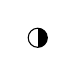
\begin{tikzpicture}
    \fill[black] (0,0) -- (0,0.8ex) arc[start angle=90,end angle=-90,radius=0.8ex] -- cycle;
    \fill[white] (0,0) -- (0,0.8ex) arc[start angle=90,end angle=270,radius=0.8ex] -- cycle;
    \draw (0,0) circle (0.8ex);
  \end{tikzpicture}%
}

\newcommand{\emptycircle}{\tikz \draw (0,0) circle (0.8ex);}

% Define commands for the squares
\newcommand{\darksquare}{%
    
\begin{tikzpicture}[scale=0.5]
        \fill[black] (0,0) rectangle (0.4,0.4);
    \end{tikzpicture}%
}

\newcommand{\lightsquare}{%
    
\begin{tikzpicture}[scale=0.5]
        \fill[gray] (0,0) rectangle (0.4,0.4);
    \end{tikzpicture}%
}

\newcommand{\halfsquare}{%
    
\begin{tikzpicture}[scale=0.5]
        \fill[gray] (0,0) rectangle (0.2,0.4);
        \fill[black] (0.2,0) rectangle (0.4,0.4);
    \end{tikzpicture}%
}

\newcolumntype{P}{>{\hspace{0.3cm}}p{0.9cm}}
\newcolumntype{C}{>{\centering\arraybackslash}m{3cm}}  % Category column
\newcolumntype{X}{>{\centering\arraybackslash}m{4cm}}  % Attack column


\hyphenation{op-tical net-works semi-conduc-tor IEEE-Xplore}

\newcommand{\paragrabf}[1]{\noindent \textbf{#1}\ }

\usepackage{titlesec}
\titlespacing{\section}{0pt}{*0.8}{*0.5}
\titlespacing{\subsection}{0pt}{*0.5}{*0.3} % Adjust spacing before and after % shorten the paper and then remove

%%%%%%From ISCA



%%%End of ISCA


\begin{document}

%\title{A Novel Side-Channel Vulnerability in Intel AMX}


% \thanks{Manuscript received November 4, 2023; revised February 28, 2024.}
% \thanks{The next few paragraphs should contain 
% the authors' current affiliations, including current address and e-mail. For 
% example, First A. Author is with the National Institute of Standards and 
% Technology, Boulder, CO 80305 USA (e-mail: author@boulder.nist.gov). }
% \thanks{Second B. Author and Third C. Author are with Rice University, Houston, TX 77005 USA. (e-mail: authorB@lamar.colostate.edu, authorC@abc.com).}
% }

% The paper headers
% \markboth{IEEE Journal of \LaTeX\ Class,~Vol.~12, No.~6, February~2024}%
% {Shell \MakeLowercase{\textit{et al.}}: A Sample Article Using IEEEtran.cls for IEEE Journals}

% \IEEEpubid{0000-0000~\copyright~2024 IEEE}
% Remember, if you use this you must call \IEEEpubidadjcol in the second
% column for its text to clear the IEEEpubid mark.

 \maketitle

 %\input{Shorts/Intro-short}

\begin{spacing}{0.96}
    
\begin{abstract}
Retrieval-Augmented Generation (RAG) is often used with Large Language Models (LLMs) to infuse domain knowledge or user-specific information. In RAG, given a user query, a retriever extracts chunks of relevant text from a knowledge base. These chunks are sent to an LLM as part of the input prompt. Typically, any given chunk is repeatedly retrieved across user questions. However, currently, for every question, attention-layers in LLMs fully compute the key values (KVs) repeatedly for the input chunks, as state-of-the-art methods cannot reuse KV-caches when chunks appear at arbitrary locations with arbitrary contexts. Naive reuse leads to output quality degradation.  This leads to potentially redundant computations on expensive GPUs and increases latency. In this work, we propose \sys, a system for managing and reusing precomputed KVs corresponding to the text chunks (we call \textit{chunk-caches}) in RAG-based systems. We present how to identify \hl{\textit{chunk-caches} that are reusable}, how to efficiently perform a small fraction of recomputation to \textit{fix} the cache to maintain output quality, and how to efficiently store and evict \textit{chunk-caches} in the hardware for maximizing reuse while masking any overheads. With real production workloads as well as synthetic datasets, we show that \sys reduces redundant computation by \textbf{51\%} over SOTA prefix-caching and \textbf{75\%} over full recomputation.
\hl{Additionally, with continuous batching on a real production workload, we get a \textbf{1.6$\times$} speedup in throughput and a \textbf{2$\times$} reduction in end-to-end response latency over prefix-caching while maintaining quality, for both the \llama-3-8B and \llama-3-70B models. 
}
\end{abstract}






\begin{IEEEkeywords}
Intel Advanced Matrix Extensions (AMX), Value-dependent timing side-channel, ML privacy, NN sparsity.
\end{IEEEkeywords}

\section{Introduction}
%\IEEEPARstart{P} 
Privacy of machine learning models deployed on Machine Learning as a Service (MLaaS) platforms can be compromised by 
%have been facing growing scrutiny due to significant vulnerabilities that attackers can exploit to compromise critical aspects of these systems. These vulnerabilities allow 
adversaries to extract sensitive details, including model architecture
and hyperparameters~\cite{TramerZJRR16}. 
%, which are often proprietary and essential to the performance and commercial value of the model.
%These attacks are often based on gradient based inference, path-searching and surrogate model training methods to leak the target data. Adversary can train shadow models based on the output of the target model and then based on the confidence score leak the members on which model is trained.
%Trusted Execution Environments (TEEs) offer a secure enclave within a processor, safeguarding sensitive data and code from unauthorized access, even if the operating system is compromised. They protect against threats such as malicious software and physical attacks such as memory bus snooping. The CPU acts as the root of trust, establishing secure enclaves with hardware-enforced encryption and attestation. Intel SGX is a prime example, creating isolated "enclaves". TEEs like SGX are increasingly used to secure ML models (e.g., Slalom \cite{tramèr2019slalomfastverifiableprivate}, DarkneTZ \cite{Mo2020DarkneTZ}, TEESlice \cite{li2024teesliceprotectingsensitiveneural}, Occlumency \cite{Lee2019Occlumency}). These works leverage TEEs to protect sensitive computations and data within isolated enclaves, mitigating model stealing and unauthorized access risks. Being more efficient than cryptographic techniques, TEEs are being utilized as the root of trust by most current MLaaS applications to secure ML models.
% \begin{comment}
% *** Commenting Original Text***
% However, we show that as hardware accelerators become more deeply embedded %\cite{jeong2021rasa,jeong2023vegeta,nassif2022sapphire 
% \cite{intel2023amx}, they bring unique challenges for AI security that existing research has yet to explore fully. We show that the tight integration of on-core AI accelerators like Intel AMX  introduces a timing side channel that bypasses conventional defenses like speculative execution mitigations %~\cite{yan2018invisispec}
% or cache isolation %~\cite{kiriansky2018dawg}
% .
% \end{comment}
However, this paper shows that 
%as hardware accelerators become more deeply embedded %\cite{jeong2021rasa,jeong2023vegeta,nassif2022sapphire 
%\cite{intel2023amx}, they bring unique challenges for AI security that existing research has yet to explore fully. We show that
the tight integration of on-core AI accelerators like Intel AMX\cite{intel2023amx} causes AMX performance to depend upon operand value which works as proxy, enabling timer attacks on ML models thus introducing a timing side channel that bypasses conventional defenses like speculative execution mitigations %~\cite{yan2018invisispec}
or cache isolation %~\cite{kiriansky2018dawg}
and challenges the architectural and data privacy of ML.

\begin{comment}

Intel AMX's versatility supports both training and inference workloads in AI applications. Bfloat16 operations balance precision and dynamic range, making them suitable for neural network training, %~\cite{googleBFloat16Secret} 
while 8-bit integer operations enhance inference performance with negligible accuracy loss, providing significant acceleration for modern AI workloads. 
    
\end{comment}

\begin{comment}
*** Commenting Original Text***
We show that AMX performance depends on an operand value.
%as shown in Figure~\ref{fig:Cumulative_execution_time}.   
This dependency works as a proxy that
extends beyond traditional side channels, enabling timer attacks on machine learning models that challenge the architectural and data privacy of ML. 

\end{comment}



%\subsection{Microarchitectural Side Channel Attacks}
%\textbf{Transmission Channels.} 
Cache attacks exploit timing variations between accessing or flushing data in cache levels or DRAM~\cite{GrussFlushFlush}.
%.Prime+Probe%~\cite{prime_probe}
%, Flush+Reload%~\cite{flush+reload}
%, and Flush+Flush
 %\textcolor{red}{1 cite? }rely on cache set monitoring or eviction timing.
Spectre~\cite{kocher2020spectre} and Meltdown~\cite{meltdown} exploit speculative execution and exception handling. 
%Variants like Foreshadow %~\cite{van2018foreshadow} and LVI %~\cite{lvi} breach SGX and inject malicious data. %RIDL%~\cite{ridl}, Fallout%~\cite{canella2019fallout}, and Zombieload%~\cite{schwarz2019zombieload}
MDS Attacks~\cite{schwarz2019zombieload,canella2019fallout} target microarchitectural buffers. Defenses include cache partitioning~\cite{kiriansky18dawg}, 
%~\cite{herdrich2016cache,kiriansky18dawg}
Invisispec~\cite{yan2018invisispec}, privileged access controls (e.g., RAPL restrictions)~\cite{Lipp2021Platypus}, SMT disabling and other patches with performance overhead. 
%, and TurboBoost mitigation. 
%~\cite{wang2022hertzbleed}. 
%
However, no work has been done on the security evaluation of newly built Intel AMX for AI applications.


% \noindent\textbf{Speculative and Transient-Execution Attacks.}  %NetSpectre~\cite{schwarz2019netspectre} demonstrates remote speculative attacks using AVX timing.



%\subsection{Attacks on ML}
%\noindent\textbf{Model and Hyperparameter Extraction.} 
Black-box attacks extract model functionality or hyperparameters with minimal access but require confidence scores and are mitigated by  various methods like limiting the query rate, obfuscating the input data by masking, rounding confidence, or using homomorphic encryption.  
%Model inversion attacks~\cite{Fredrikson2015ModelInversion,Wand2022VarModelInversion} reconstruct sensitive inputs such as facial images.
%\noindent\textbf{Physical and Microarchitectural Attacks on ML.} 
Early physical attacks, such as IKWYS~\cite{wei2018know}  %and CSI NN~\cite{CSINN2018}, 
used power or EM side channels to infer neural network (NN) parameters but required physical access. %. Cache Telepathy
~\cite{Yan2020Cachetelepathy} 
%and DeepRecon~\cite{HongDeepRecon2018} 
leverages cache timing to leak NN architecture but is reliant on particular ML libraries and co-location. 
%Rowhammer-based attacks like DeepSteal~\cite{RakinDeepSteal2021} leak partial weights but assume partial black-box knowledge~\textcolor{red}
 We confirmed that vulnerabilities on NNs using floating-point timing~\cite{9218707} have been completely mitigated in the Intel AMX design and thus are no longer available to the attacker. 
%Despite advances, non-cache based microarchitectural side-channel attacks targeting NN parameters remain unexplored.

%  Traditionally, power side-channel attacks require physical access to a system to measure power consumption or electromagnetic emissions. Such attacks are less common and practical because they require a high level of access. However, Lipp et al. \cite{Lipp2021Platypus} demonstrated a method to exploit the Running Average Power Limit (RAPL) interface for power side-channel attacks without needing physical access. However, RAPL is now a privileged interface, making this technique inaccessible to the unprivileged attacker. 
% %
% Dynamic Voltage and Frequency Scaling (DVFS), an optimization technique for power management, can paradoxically open up new attack surfaces by converting power side channels into timing attacks. This vulnerability was exploited in Hertzbleed \cite{wang2022hertzbleed} to leak data by throttling under power limits, and in Collide+Power \cite{kogler2023collide+}, where power limits and throttling were manipulated to convert the memory power side channels into timing variations. Notably, power limit controls are usually privileged, and throttling can be mitigated by disabling Turbo Boost. As such, our work reveals a new, generic vulnerability in Intel AMX, specifically within its power and performance management mechanisms. Interestingly, unlike DVFS-related vulnerabilities, our discovered vulnerability persists irrespective of DVFS states and allows for exploitation regardless of whether DVFS is on or off. Additionally, our attack does not require a shared cache—unlike Collide+Power, which necessitates shared cache access to leak data, is now patched and leaks significantly lower rate (4.82 compared to 76.8 bits per hour for our attack).

 In this paper, we demonstrate the feasibility of exploiting Intel AMX 
 %this newly discovered vulnerability in NN operations 
 to leak sensitive information in NN, such as sparsity of it's weights. Inferring sparsity could inadvertently reveal sensitive data patterns. Understanding the sparsity pattern might provide insights into the underlying data distributions, potentially breaching data privacy.
Additionally, knowledge of sparsity patterns could enable attackers to craft more effective adversarial attacks. By understanding the structure of a model, an attacker might design inputs that strategically exploit sparsity, leading to degraded model performance or incorrect predictions.
 %Previous works in the literature have targeted NN models to infer architectural details, inputs, and weights, often necessitating physical access for power and electromagnetic measurements \cite{CSINN2018} or shared cache manipulation via known cache side channels \cite{Yan2020Cachetelepathy}.  
 Our approach is notable for not requiring physical access or a shared cache, unlike previous works %in the literature have targeted NN models to infer architectural details, inputs, and weights, 
 that often necessitating physical access for power and electromagnetic measurements 
 %\cite{CSINN2018} 
 or shared cache manipulation via known cache side channels \cite{Yan2020Cachetelepathy}, lowering the bar for potential attackers.
%Specifically, we investigate the behavior of AMX multiplication.
%, which operates in five distinct states and fluctuates between 52 and 20,000 cycles. 
We discover that the execution times of the Intel AMX multiplications vary depending on the operand's value. 
%are not consistent when AMX is transitioning between different states. 
%However, t
\begin{comment}
This phenomenon is different from the observed Hertzbleed~\cite{wang2022hertzbleed} because our attack continues to function even with the Intel Turbo Boost (DVFS) feature turned off, suggesting a novel root cause specific to the Intel AMX design compared to the Hertzbleed that relies on DVFS feature enabled and obsolete cryptographic libraries. 
\end{comment}
% New
This phenomenon is different from the observed Hertzbleed\cite{wang2022hertzbleed, liu2022frequency}, which is a side-channel attack that leverages dynamic voltage and frequency scaling (DVFS) on modern x86 processors to transform power fluctuations into timing attacks, extractable without direct power measurement. Hertzbleed exploits CPU frequency variations, linked to data-dependent power consumption. Our attack continues to function even with the Intel Turbo Boost (DVFS) feature turned off, suggesting a novel root cause specific to the Intel AMX design compared to Hertzbleed, which relies on the DVFS feature being enabled and obsolete cryptographic libraries.
Our attack also bypasses TEE based defenses in contrary to Rowhammer-based attacks like DeepSteal~\cite{RakinDeepSteal2021} that leak partial weights but can be protected by TEE-based defenses. 
%assume partial black-box knowledge

%Particularly, after exiting high-latency states and before stabilizing to a steady state, the execution time becomes a data-dependent process. 
%This dependency arises because 

%Our reverse engineering suggests that Intel AMX has a separate clock from the CPU clock and skipping the zero values in the multiplication operands of the accelerator influence the trend of frequency adjustments by leading to less power consumption, creating exploitable and unique timing differences.
%
%We demonstrate the exploitation of this side-channel vulnerability, showing that the execution time of AMX multiplications can be systematically measured to infer the sparsity of hidden weights of a NN. In this first study,
%our practical example, 
We successfully leaked zeros in 64 hidden weights with 100\% accuracy within 50 minutes of observation without access to the NN output value, confidence score or shared cache bypassing state of the art defenses such as obfuscation, masking or rounding confidence values of NN and cache defenses.
% 
Our proof of concept (PoC) attack  (\textsc{Thor}) represents the first step toward a new direction in ML privacy attacks. It is an attack on a single-layer NN but its significance is that, unlike prior approaches that rely on {{confidence scores}}, logits,  physical access, or higher privilege, \textsc{Thor} leverages timing information alone to infer critical and private parameters like NN's weight sparsity patterns and distributions. 
%Thor is fast but is limited to a single layer NN.

This paper presents the following contributions:
\begin{compactitem}
\item It characterized and reverse-engineered the Intel AMX, 
% data-dependent timing 
uncovering 
%its unique exploitable properties of Intel AMX features
%\item It identifies 
a novel type of data-dependent timing side-channel vulnerability within the Intel AMX accelerator.

\item It demonstrates the techniques necessary to exploit this newly discovered timing side-channel for launching attacks on NNs. Specifically, it illustrates how to determine the sparsity of NN weights by measuring execution time.
We show that the \textsc{Thor} leakage rate is 631\% and 1,493\% higher than the maximum leakage rates in the Hertzbleed and Collide+Power~\cite{kogler2023collide+} attacks, respectively.
\item We discuss defenses, propose a counter-measurement and measure its overhead on power consumption (2.59\% to 12.33\%).   
\end{compactitem}
\vspace{0.1em}
\textbf{Responsible disclosure.}  We reported our attack and findings to Intel in May 2024 and Intel confirmed our findings. %Moreover, we are planning to open source our code.




% \section{Background \& Related Works}
% \subsection{}
% The discoveries of Spectre \cite{kocher2019spectre} and Meltdown \cite{meltdown} showed how speculative execution and architectural optimizations could be exploited in the form of side  channels exposing private data through the foundations of optimization and subtle timing differences. Subsequent research 
% uncovered an avalanche of vulnerabilities targeting various micro-architectural components such as 
% %on other atta~\cite{pandorasbox} 
% caches ~\cite{prime_probe, flush+reload, GrussFlushFlush, osvik2006cache}, internal CPU buffers ~\cite{kocher2019spectre,Phantom2023,spectre_here_to_stay2019, SpectreV4,kiriansky2018speculative,koruyeh2018spectre,maisuradze2018ret2spec,meltdown, canella2018systematic,van2018foreshadow,lvi, moghimi2020medusa,ridl,
% schwarz2019zombieload, canella2019fallout, moghimi2023downfall}, prefetcher ~\cite{gruss2016prefetch,lipp2022amd,augury,gofetch2024}, PACMAN~\cite{PACMAN}, TLB ~\cite{Tatar2022tlbdr,gras_translation_2018,koschel2020tagbleed}, port contention~\cite{bhattacharyya2019smotherspectre}, scheduler queues~\cite{SQUIP2023}, micro-op cache~\cite{uop2021Ashish}, exploiting other shared micro-architectural components~\cite{CrossTalk2021, weber2021osiris} and remote attacks~\cite{Brumley2003Remote,Bernstein2005,Aciicmez2007d,Crosby2009,Beery2013TIME,VanHoef2016Heist,VanGoethem2020Timeless,Irazoqui2015Lucky,schwarz2019netspectre,schwarzl2023practical, Schwarzl2022Remote,Gruss2019page,Kurt2020Netcat, wang2022hertzbleed,Zhao2009cache},   fundamentally reshaped our understanding of processor security. 

% However, no work has been done on security evaluation of Intel AMX.  

% \subsection{Intel AMX Architecture and Instructions.}
% Intel AMX is an integrated accelerator introduced with the 4th Gen Intel Xeon Scalable processors, specifically engineered to boost the efficiency of matrix computations. %Figure~\ref{fig:AMX-arch} illustrates the Intel AMX architecture.

% AMX introduces a new set of registers and instructions. The registers in Intel AMX are known as Tiles, a new concept in Intel CPUs that provide a matrix of data registers, as opposed to the traditional vector registers seen in previous SIMD architectures like AVX-512. AMX includes 8 Tile registers, each capable of holding up to 16 rows with 64 bytes per row, amounting to a total of 1 KB per Tile. The number of rows and the number of bytes per row can be adjusted using the LDTILECFG instruction, and this configuration information is stored as metadata in a control register known as TILECFG. Once this configuration is set, AMX instructions such as load, store, and matrix multiplication will operate according to the specified dimensions for each Tile. Intel AMX instructions are synchronized with the Intel Architecture host (IA host) instruction stream, and the Tile loads and stores are coherent with the host memory \cite{Intel_Arc_Ins_Set_Extensions}.

% Tile Matrix Multiply unit (TMUL) serves as the accelerator engine for executing multiplication calculations. When using full-size Tile operands, the latency of the multiplication instruction is 52 cycles, while pipelining allows for a throughput of 16 cycles. Intel AMX supports two data types: BF16 and INT8. Consequently, it can perform 512 multiplications and 512 additions per cycle for BF16 and 1024 multiplications and 1024 additions per cycle for INT8 \cite{IntelOptRefManual}. 

\begin{comment}
AMX instructions utilize port 5 as their dedicated execution port. When two hyper-threads are active within a core, they compete for the same resources to execute AMX instructions.
\end{comment}

% \subsection{Microarchitectural Side Channel Attacks}
% %\textbf{Transmission Channels.} 
% Cache attacks exploit timing variations between cache levels or DRAM. Prime+Probe%~\cite{prime_probe,osvik2006cache}
% , Flush+Reload%~\cite{flush+reload}
% , and Flush+Flush~\cite{GrussFlushFlush} rely on cache set monitoring or eviction timing.  Spectre~\cite{kocher2020spectre} and Meltdown~\cite{meltdown} exploit speculative execution and exception handling. Variants like Foreshadow %~\cite{van2018foreshadow} 
% and LVI %~\cite{lvi} 
% breach SGX and inject malicious data. RIDL %~\cite{ridl}
% , Fallout%~\cite{canella2019fallout}
% , and Zombieload %~\cite{schwarz2019zombieload} 
% target microarchitectural buffers. Defenses include cache partitioning
% %~\cite{herdrich2016cache,kiriansky18dawg}
% , Invisispec
% %~\cite{Invisispec}
% , privileged access controls (e.g., RAPL restrictions), SMT disabling, and TurboBoost mitigation. 
% %~\cite{wang2022hertzbleed}. 

% However, no work has been done on security evaluation of Intel AMX.


% % \noindent\textbf{Speculative and Transient-Execution Attacks.}  %NetSpectre~\cite{schwarz2019netspectre} demonstrates remote speculative attacks using AVX timing.



% \subsection{Attacks on ML}
% %\noindent\textbf{Model and Hyperparameter Extraction.} 
% Black-box attacks extract model functionality~\cite{TramerZJRR16,Orekondy18Knock} or hyperparameters~\cite{wang2018hyperparameters} with minimal access but require confidence scores and are mitigated by  various methods \textcolor{red}{TODO}. 
% %Model inversion attacks~\cite{Fredrikson2015ModelInversion,Wand2022VarModelInversion} reconstruct sensitive inputs such as facial images.
% %\noindent\textbf{Physical and Microarchitectural Attacks on ML.} 
% Early physical attacks, such as IKWYS~\cite{wei2018know} and CSI NN~\cite{CSINN2018}, used power and EM side-channels to infer neural network (NN) parameters but require physical access. Cache Telepathy~\cite{Yan2020Cachetelepathy} and DeepRecon~\cite{HongDeepRecon2018} leverage cache timing to leak NN architecture but are reliant on particular ML libraries and co-location. Rowhammer-based attacks like DeepSteal~\cite{RakinDeepSteal2021} leak partial weights but assume partial black-box knowledge.
%  We confirmed that attacks on neural networks using floating-point timing vulnerabilities~\cite{9218707} have been largely mitigated by modern accelerators such as Intel AMX. %Recent attacks like DeepRecon~\cite{HongDeepRecon2018} focus on architecture and parameter extraction but fail to address MIA comprehensively.

% Despite advances, direct microarchitectural side-channel attacks targeting neural network parameters remain unexplored.

\section{Threat Model}
The attacker and victim are two distinct processes running on the same server. These processes are entirely isolated in terms of address space and can be executed on different CPU cores. As shown in Figure \ref{fig:Thor-threat-model}, the victim process is an API that runs a NN designed for specific tasks and utilizes Intel AMX for matrix computations. The attacker process, which operates as a non-privileged user, does not have direct access to the model’s parameters but interacts with the model via the inference API. The attacker sends crafted inputs to the inference API and measures the timing of the victim process's responses. By examining timing variations, the attacker can gain insights into the NN's internal parameters by taking advantage of the timing differences caused by Intel AMX computations. We assume cache defenses are deployed or there is no shared cache,  thus channels such as \cite{Yan2020Cachetelepathy} is not available to the adversary. The ML model is a single layer NN protected by obfuscated the confidence score and the output by methods such as adding noise or rounding confidence scores \cite{Fredrikson2015ModelInversion}. The victim may leverage TEEs, Intel SGX, to execute the NN computations within isolated enclaves.


% \textsc{Thor} exploits Intel AMX timing variations to infer sparsity patterns in neural network weights hosted on inference APIs. As a non-privileged attacker, it sends tailored inputs and measures response times, leveraging amplified timing differences in AMX Warm-State transitions to detect zero weights.
% % The attack works for both binary and non-binary weight patterns without requiring confidence scores, logits, or training data. It is adaptable to diverse environments, including cloud systems, MLaaS platforms, and SGX enclaves. By avoiding reliance on shared memory or privileged interfaces (for example, Flush + Reload, PlatyPus), and speculative or physical access attacks (for example, Specter, EM based methods), \textsc{Thor} offers a purely timing-based approach. Thor is limited to a single-layer neural network.

\begin{figure}[!ht] %\vspace{-5mm}
    \centering
   \includegraphics[width=\linewidth]{images/threat_model_v4.pdf} 
    \caption{\textsc{Thor} Threat Model.}
    \label{fig:Thor-threat-model}
\end{figure}


% %{System Configuration.} 
% Our investigations utilized a server running {Red Hat Enterprise Linux release 9.4} with {Linux kernel version 5.14}, powered by an { Intel Xeon Gold 5420+} from the {Sapphire Rapids microarchitecture}. 
% %
% The tests were carried out with a range of configurations,
% %shown in Table~\ref{tab:configurations}, 
% including the { autonomous (hardware-only)} and { cooperative P-state control modes}, under {minimal power}, {maximum performance}, and {efficiency-focused} platform power settings. {Turbo Boost} was tested in both {enabled} and {disabled states}. {Prefetchers} were toggled between {enabled} and {disabled states} across experiments to assess their impact on noise and timing variations. The server configurations included the UEFI firmware versions SRV650-v3-3.14 (May 2024) and SRV650-v3-3.20 (June 2024), with the latter mitigating certain Spectre variants but remaining vulnerable to our attack, \textsc{Thor}.

\vspace{-1em}\section{Thor}
%{System Configuration.} 
Our investigations utilized a server running {Red Hat Enterprise Linux release 9.4} with {Linux kernel version 5.14}, powered by an { Intel Xeon Gold 5420+} from the {Sapphire Rapids microarchitecture}. 
%
The tests were carried out with a range of configurations,
%shown in Table~\ref{tab:configurations}, 
including the { autonomous (hardware-only)} and { cooperative P-state control modes}, under {minimal power}, {maximum performance}, and {efficiency-focused} platform power settings. {Turbo Boost} was tested in both {enabled} and {disabled states}. {Prefetchers} were toggled between {enabled} and {disabled states} across experiments to assess their impact on noise and timing variations. The server configurations included the UEFI firmware versions SRV650-v3-3.14 (May 2024) and SRV650-v3-3.20 (June 2024), with the latter mitigating certain Spectre variants but all above settings remains vulnerable to our attack. 
%, \textsc{Thor}.

%\subsection{Intel AMX Architecture and Instructions.}
\subsection{Reverse Engineering}
Intel AMX is an on-core accelerator introduced with the 4th Gen Intel Xeon Scalable processors, specifically engineered to boost matrix computation efficiency.
%Figure~\ref{fig:AMX-arch} illustrates the Intel AMX architecture.
%
%AMX introduces a new set of registers and instructions. The registers in Intel AMX are known as Tiles, a new concept in Intel CPUs that provides a matrix of data registers, as opposed to the traditional vector registers seen in previous SIMD architectures like AVX-512. AMX includes eight Tile registers, each capable of holding up to 16 rows with 64 bytes per row, amounting to 1 KB per Tile. 
%The number of rows and the number of bytes per row can be adjusted using the LDTILECFG instruction, and this configuration information is stored as metadata in a control register known as TILECFG. Once this configuration is set, AMX instructions such as load, store, and matrix multiplication will operate according to the specified dimensions for each Tile. Intel AMX instructions are synchronized with the Intel Architecture host (IA host) instruction stream, and the Tile loads and stores are coherent with the host memory \cite{Intel_Arc_Ins_Set_Extensions}.
Tile Matrix Multiply unit (TMUL) is the accelerator engine for executing multiplication calculations. 
%When using full-size Tile operands, the latency of the multiplication instruction is 52 cycles, while pipelining allows for a throughput of 16 cycles. 
%Intel AMX supports two data types: BF16 and INT8. Consequently, it  Intel AMX can perform 512 multiplications and 512 additions per cycle for BF16 and 1024 multiplications and 1024 additions per cycle for INT8 \cite{IntelOptRefManual}. 
Intel AMX can perform 512 and 1024 multiplications/additions per cycle for BF16 and INT8, respectively~\cite{IntelOptRefManual}. 
% \subsection{Dynamic Power/Performance Vulnerabilities of Intel AMX}
%In this section we explore AMX features that have the potential to be exploited in a transmission channel part of a microarchitectural attack.x

%








% \begin{tcolorbox}[ colback=lightgray!20,
% colframe=gray!50,
% boxrule=0.3mm,
% arc=2mm,
% width=0.48\textwidth,
% sharp corners=all, left=2mm,
% right=2mm,
% top=1mm,
% bottom=1mm
% ] These findings demonstrate that Intel AMX includes a frequency management unit that controls the operating frequency of the TMUL accelerator. This unit can potentially access or create frequencies that differ from the CPU frequency as shown as Transition Behavior of AMX Frequency to CPU Frequency in Warm State. 
% This finding is in contrast to the root cause known for AVX performance variation, known as power up/down~\cite{netspectre} which does not vary to match  the core frequency.  
% \end{tcolorbox}

%\begin{figure}[!hbp]
%\centering\includegraphics[width=0.4\textwidth]{images/Freq_transition.pdf}
%\caption{Illustration of AMX Frequency Adjustment During Transition Periods: (a) shows the transition to a 1.2 GHz CPU frequency, with intermediate operation at 1 GHz; (b) demonstrates the adjustment to a 2 GHz CPU frequency, passing through 1 GHz and 1.3 GHz stages.}
%\label{fig:Freq_transition}
%\end{figure}
%{\color{blue} Put Freq\_transition figure here}



% \begin{figure}[ht!]
%     \centering
%     \begin{tikzpicture}
%         \begin{axis}[
%             font=\scriptsize,
%             width=\linewidth*0.7,
%             height=\linewidth*0.32,
%             bar width=50,
%             xmin=21800, xmax=24650,
%             ybar,
%             ylabel={Frequency},
%             ylabel style={yshift=0pt},
%             ymin=0, ymax=0.006,
%             legend style={
%                 legend columns=1, 
%                 at={(1.01,0.5)}, 
%                 anchor=west,   
%                 font=\tiny,
%             },
%             legend image code/.code={\draw[fill=#1,draw=none] (0cm,-0.1cm) rectangle (0.25cm,0.1cm);},
%             legend entries={100\% sparsity, 50\% sparsity, 0\% sparsity}
%         ]
%             \addplot+[hist={density, bins=50}, fill=lightgray, draw=none] table[y index=0] {Diagrams/Data/100-0.txt};
%             \addplot+[hist={density, bins=50}, fill=black, draw=none] table[y index=0] {Diagrams/Data/100-half.txt};
%             \addplot+[hist={density, bins=50}, fill=gray, draw=none] table[y index=0] {Diagrams/Data/100-1.txt};
%         \end{axis}
%         \node[anchor=south east] at (rel axis cs:-0.05,1) {(a)};
%     \end{tikzpicture}
%     \begin{tikzpicture}
%         \begin{axis}[
%             font=\scriptsize,
%             width=\linewidth*0.7,
%             height=\linewidth*0.32,
%             bar width=50,
%             xmin=35500, xmax=56000,
%             ybar,
%             ylabel={Frequency},
%             ylabel style={yshift=0pt},
%             ymin=0, ymax=0.00205,
%             legend style={
%                 legend columns=1, 
%                 at={(1.01,0.5)}, 
%                 anchor=west,   
%                 font=\tiny,
%             },
%             legend image code/.code={\draw[fill=#1,draw=none] (0cm,-0.1cm) rectangle (0.25cm,0.1cm);},
%             legend entries={100\% sparsity, 50\% sparsity, 0\% sparsity}
%         ]
%             \addplot+[hist={density, bins=60}, fill=lightgray, draw=none] table[y index=0] {Diagrams/Data/1000-0.txt};
%             \addplot+[hist={density, bins=60}, fill=black, draw=none] table[y index=0] {Diagrams/Data/1000-half.txt};
%             \addplot+[hist={density, bins=60}, fill=gray, draw=none] table[y index=0] {Diagrams/Data/1000-1.txt};
%         \end{axis}
%         \node[anchor=south east] at (rel axis cs:-0.05,1) {(b)};
%     \end{tikzpicture}
%     \begin{tikzpicture}
%         \begin{axis}[
%             font=\scriptsize,
%             width=\linewidth*0.7,
%             height=\linewidth*0.32,
%             bar width=50,
%             xmin=170000, xmax=345000,
%             xlabel={Execution time (cycle)},
%             ybar,
%             ylabel={Frequency},
%             ylabel style={yshift=0pt},
%             ymin=0, ymax=0.00022,
%             legend style={
%                 legend columns=1, 
%                 at={(1.01,0.5)}, 
%                 anchor=west,   
%                 font=\tiny,
%             },
%             legend image code/.code={\draw[fill=#1,draw=none] (0cm,-0.1cm) rectangle (0.25cm,0.1cm);},
%             legend entries={100\% sparsity, 50\% sparsity, 0\% sparsity}
%         ]
%             \addplot+[hist={density, bins=60}, fill=lightgray, draw=none] table[y index=0] {Diagrams/Data/10000-0.txt};
%             \addplot+[hist={density, bins=60}, fill=black, draw=none] table[y index=0] {Diagrams/Data/10000-half.txt};
%             \addplot+[hist={density, bins=60}, fill=gray, draw=none] table[y index=0] {Diagrams/Data/10000-1.txt};
%         \end{axis}
%         \node[anchor=south east] at (rel axis cs:-0.05,1) {(c)};
%     \end{tikzpicture}
% \caption{Data Dependent AI computation: Cumulative Execution Time of Programs with varying zero bits in the TMUL operand of Intel AMX.}
% \label{fig:Cumulative_execution_time}
% \end{figure}

%\subsection{Non-speculative Value-based Vulnerability}

%\subsubsection{Value Dependency of Transition Time} \label{sec:valuedependencyofTransitionTime}
We studied the impact of operand sparsity on TMUL operations. % in Warm State.
%In our investigation of the TMUL execution time transition in the Warm State, we discovered an interesting effect involving zero values in the Tile operands during multiplication. 
By varying the number of zero values in the Tile operands during multiplication, we observed that increasing the number of zeros accelerates the 
AMX execution. 
%transition period. 
This effect is illustrated in Figure~\ref{fig:Cumulative_execution_time}
%\ref{fig:Effect_of_zeros_on_transition}
, which presents three distinct distributions showing the sparsity levels of the operand: 100\% sparsity, 50\% sparsity, and 0\% sparsity. 
The results indicate that a greater sparsity of operands in the tile operands leads to faster 
execution of the TMUL. The program with 1,000 AMX multiplications averages 54,005 cycles when operands have 0\% sparsity. Increasing sparsity to 50\% and 100\% reduces the average execution time to 45,953 and 38,747 cycles, respectively. In this case, 50\% and 100\% more sparsity make the execution 17.5\% and 39.4\% faster, respectively.
%Consequently, the execution time of a program that utilizes AMX multiplications is closely associated with the sparsity of its input operands. In Figure \ref{fig:Cumulative_execution_time}, we demonstrate this relationship 
%by executing 
%three test programs with 100, 1000, and 10,000 AMX multiplications, each 
%with varying levels of tile operand sparsity (0\%, 50\%, and 100\%). Each scenario was executed 1,000 times to construct the histogram. Our results reveal that varying sparsity levels significantly impact the execution time of AMX multiplications, with increased sparsity leading to faster program execution.
%

\begin{figure}[htbp!]
    \centering
    % \begin{tikzpicture}
    %     \begin{axis}[
    %         font=\scriptsize,
    %         width=\linewidth*0.95,
    %         height=\linewidth*0.35,
    %         bar width=50,
    %         xmin=21800, xmax=24650,
    %         xlabel={Execution time (cycle)},
    %         ybar,
    %         ylabel={Frequency},
    %         ylabel style={yshift=-15pt},
    %         ymin=0, ymax=0.006,
    %         legend style={
    %             at={(0.5,1)}, 
    %             anchor=north, 
    %             legend columns=-1,
    %             font=\scriptsize,
    %             /tikz/column 2/.style={column sep=5pt}, 
    %             fill=none,
    %             draw=none
    %         },
    %         legend image code/.code={\draw[fill=#1,draw=none] (0cm,-0.1cm) rectangle (0.25cm,0.1cm);},
    %         legend entries={100\% sparsity, 50\% sparsity, 0\% sparsity}
    %     ]
    %         \addplot+[hist={density, bins=50}, fill=lightgray, draw=none] table[y index=0] {Diagrams/Data/100-0.txt};
    %         \addplot+[hist={density, bins=50}, fill=black, draw=none] table[y index=0] {Diagrams/Data/100-half.txt};
    %         \addplot+[hist={density, bins=50}, fill=gray, draw=none] table[y index=0] {Diagrams/Data/100-1.txt};
    %     \end{axis}
    %     \node[anchor=south east] at (rel axis cs:-0.05,1) {(a)};
    % \end{tikzpicture}
    \begin{tikzpicture}
        \begin{axis}[
            font=\scriptsize,
            width=\linewidth*0.95,
            height=\linewidth*0.35,
            bar width=50,
            xmin=35500, xmax=56000,
            xlabel={Execution time (cycle)},
            ybar,
            ylabel={Frequency},
            ylabel style={yshift=-15pt},
            ymin=0, ymax=0.0024,
            legend style={
                at={(0.5,1)}, 
                anchor=north, 
                legend columns=-1,
                font=\scriptsize,
                /tikz/column 2/.style={column sep=5pt}, 
                fill=none,
                draw=none
            },
            legend image code/.code={\draw[fill=#1,draw=none] (0cm,-0.1cm) rectangle (0.25cm,0.1cm);},
            legend entries={100\% sparsity, 50\% sparsity, 0\% sparsity}
        ]
            \addplot+[hist={density, bins=60}, fill=lightgray, draw=none] table[y index=0] {Diagrams/Data/1000-0.txt};
            \addplot+[hist={density, bins=60}, fill=black, draw=none] table[y index=0] {Diagrams/Data/1000-half.txt};
            \addplot+[hist={density, bins=60}, fill=gray, draw=none] table[y index=0] {Diagrams/Data/1000-1.txt};
        \end{axis}
        %\node[anchor=south east] at (rel axis cs:-0.05,1) {(b)};
    \end{tikzpicture}
    \begin{comment}
    \begin{tikzpicture}
        \begin{axis}[
            font=\scriptsize,
            width=\linewidth*0.95,
            height=\linewidth*0.35,
            bar width=50,
            xmin=170000, xmax=345000,
            xlabel={Execution time (cycle)},
            ybar,
            ylabel={Frequency},
            ylabel style={yshift=-15pt},
            ymin=0, ymax=0.00027,
            legend style={
                at={(0.5,1)}, 
                anchor=north, 
                legend columns=-1,
                font=\scriptsize,
                /tikz/column 2/.style={column sep=5pt}, 
                fill=none,
                draw=none
            },
            legend image code/.code={\draw[fill=#1,draw=none] (0cm,-0.1cm) rectangle (0.25cm,0.1cm);},
            legend entries={100\% sparsity, 50\% sparsity, 0\% sparsity}
        ]
            \addplot+[hist={density, bins=60}, fill=lightgray, draw=none] table[y index=0] {Diagrams/Data/10000-0.txt};
            \addplot+[hist={density, bins=60}, fill=black, draw=none] table[y index=0] {Diagrams/Data/10000-half.txt};
            \addplot+[hist={density, bins=60}, fill=gray, draw=none] table[y index=0] {Diagrams/Data/10000-1.txt};
        \end{axis}
        \node[anchor=south east] at (rel axis cs:-0.05,1) {(a)};
    \end{tikzpicture}
    \end{comment}
\caption{Execution Time with Varying Operand Sparsity. }
%: Higher Sparsity Levels Lead to Faster Execution Across Different AMX Multiplications. Subfigures (a), (b), and (c) show programs with 100, 1,000, and 10,000 AMX multiplications, respectively.}

\label{fig:Cumulative_execution_time}
\end{figure}

This discovery uncovers a new value-dependent timing side channel that reveals the sparsity of Tile operands in Intel AMX. Our results suggest the presence of a zero-skipping-like mechanism for both BF16 and INT8 operands in Intel AMX design for acceleration and power saving purposes. 
%The energy consumption of the 0 matrix (100\% sparsity) is approximately \(6.45 \times 10^{-7}\) J, while the 255 matrix (0\% sparsity) consumes \(6.7 \times 10^{-7}\) J, resulting in a difference of \(0.25 \times 10^{-7}\) J. This represents a 3.88\% increase in energy consumption for the 0\% compared to the 100\% sparse weights. This observation shows a clear dependence of energy consumption on operand values. 

% \begin{figure}[ht!]
% \centering
% % \begin{tikzpicture}
% %     \begin{axis}[
% %         xlabel={Number of Instructions},
% %         ylabel={Execution Time\\(RDTSCP cycle)},
% %         legend pos=outer north east,
% %         font=\scriptsize,
% %         xlabel style={yshift=0pt},
% %         ylabel style={yshift=0pt, align=center}, 
% %         width=\linewidth*0.8,
% %         height=\linewidth*0.4,
% %         xmin= -0.1,xmax=40000,
% %         legend style={
% %                 legend columns=1, 
% %                 at={(1.01,0.5)}, 
% %                 anchor=west,   
% %                 font=\tiny,
% %             },
% %     ]
    
% %     \addplot[
% %         line width=0.8pt,
% %         color=black,
% %     ] table {Diagrams/Data/1400MHz.txt};
% %     \addlegendentry{1.2 GHz
% % CPU freq.};


% %     \addplot[
% %         line width=0.8pt,
% %         color=lightgray,
% %     ] table {Diagrams/Data/2000MHz.txt};
% %     \addlegendentry{2 GHz
% % CPU freq.};

% %     \end{axis}
    
% %     \node[darkgray, thick] at (1.7,1.4) {\scriptsize 1 GHz};
% %     \node[darkgray, thick] at (3.9,1) {\scriptsize 1.2 GHz};
% %     \node[darkgray, thick] at (1.5,0.9) {\scriptsize 1.3 GHz};
% %     \node[darkgray, thick] at (3.5,0.3) {\scriptsize 2 GHz};
% % \end{tikzpicture}
% % \caption{Illustration of AMX Frequency Adjustment During Transition Periods: The black line depicts the transition to a 1.2 GHz CPU frequency, with intermediate operation at 1 GHz; The gray line demonstrates the adjustment to a 2 GHz CPU frequency, passing through 1 GHz and 1.3 GHz stages.}
% % \label{fig:Freq_transition}
% % \vspace{1em}
% \centering
% \begin{tikzpicture}
%     \begin{axis}[
%         xlabel={Number of Instructions},
%         ylabel={Execution Time\\(RDTSCP cycle)},
%         legend pos=outer north east,
%         font=\scriptsize,
%         xlabel style={yshift=0pt},
%         ylabel style={yshift=0pt, align=center}, 
%         width=\linewidth*0.8,
%         height=\linewidth*0.4,
%         xmin= -0.1,xmax=40000,
%         legend style={
%                 legend columns=1, 
%                 at={(1.01,0.5)}, 
%                 anchor=west,   
%                 font=\tiny,
%             },
%     ]
    
%     \addplot[
%         line width=0.8pt,
%         color=black,
%     ] table {Diagrams/Data/2000_0Perc.txt};
%     \addlegendentry{0\% Sparcity};


%     \addplot[
%         line width=0.8pt,
%         color=lightgray,
%     ] table {Diagrams/Data/2000_50Perc.txt};
%     \addlegendentry{50\% Sparcity};


%     \addplot[
%         line width=0.8pt,
%         color=gray,
%     ] table {Diagrams/Data/2000_100Perc.txt};
%     \addlegendentry{100\% Sparcity};

%     \end{axis}
    
%     \node[darkgray, thick] at (0.6,0.45) {\scriptsize 1.8 GHz};
%     \node[darkgray, thick] at (1.4,1.55) {\scriptsize 1 GHz};
%     \node[darkgray, thick] at (1.5,1) {\scriptsize 1.3 GHz};
%     \node[darkgray, thick] at (3.5,0.3) {\scriptsize 2 GHz};
% \end{tikzpicture}
% \caption{Impact of Operand Sparsity on the Transition Period of TMUL Frequency: The graphs depict the transition behavior with 100\%, 50\%, and 0\% sparsity levels in the Tile operands, showing faster convergence to the CPU frequency with increased sparsity.}
% \label{fig:Effect_of_zeros_on_transition}
% \end{figure}
%\begin{figure}[!htbp]
%\centerline{\includegraphics[width=0.35\textwidth]{images/new_pic.pdf}}
%\caption{Cumulative Execution Time of Programs with Varying Operand Sparsity: The %histogram illustrates the effect of operand sparsity on program execution time, %highlighting that higher sparsity levels result in quicker execution across %different counts of AMX multiplications. Subfigures (a), (b), and (c) represent %programs with 100, 1,000, and 10,000 AMX multiplications, respectively.}
%\label{fig:Cumulative_execution_time}
%\end{figure}

%\subsection{Operand Patterns Influencing Data-Dependent Timing in AMX Multiplications.}

% \begin{figure}[htbp!]
%     \centering
%     \begin{tikzpicture}
%         \begin{axis}[
%             font=\scriptsize,
%             width=\linewidth*0.7,
%             height=\linewidth*0.32,
%             bar width=50,
%             xmin=21800, xmax=24650,
%             ybar,
%             ylabel={Frequency},
%             ylabel style={yshift=-15pt},
%             ymin=0, ymax=0.006,
%             legend style={
%                 legend columns=1, 
%                 at={(1.01,0.5)}, 
%                 anchor=west,   
%                 font=\tiny,
%             },
%             legend image code/.code={\draw[fill=#1,draw=none] (0cm,-0.1cm) rectangle (0.25cm,0.1cm);},
%             legend entries={100\% sparsity, 50\% sparsity, 0\% sparsity}
%         ]
%             \addplot+[hist={density, bins=50}, fill=lightgray, draw=none] table[y index=0] {Diagrams/Data/100-0.txt};
%             \addplot+[hist={density, bins=50}, fill=black, draw=none] table[y index=0] {Diagrams/Data/100-half.txt};
%             \addplot+[hist={density, bins=50}, fill=gray, draw=none] table[y index=0] {Diagrams/Data/100-1.txt};
%         \end{axis}
%         \node[anchor=south east] at (rel axis cs:-0.05,1) {(a)};
%     \end{tikzpicture}
%     \begin{tikzpicture}
%         \begin{axis}[
%             font=\scriptsize,
%             width=\linewidth*0.7,
%             height=\linewidth*0.32,
%             bar width=50,
%             xmin=35500, xmax=56000,
%             ybar,
%             ylabel={Frequency},
%             ylabel style={yshift=-15pt},
%             ymin=0, ymax=0.00205,
%             legend style={
%                 legend columns=1, 
%                 at={(1.01,0.5)}, 
%                 anchor=west,   
%                 font=\tiny,
%             },
%             legend image code/.code={\draw[fill=#1,draw=none] (0cm,-0.1cm) rectangle (0.25cm,0.1cm);},
%             legend entries={100\% sparsity, 50\% sparsity, 0\% sparsity}
%         ]
%             \addplot+[hist={density, bins=60}, fill=lightgray, draw=none] table[y index=0] {Diagrams/Data/1000-0.txt};
%             \addplot+[hist={density, bins=60}, fill=black, draw=none] table[y index=0] {Diagrams/Data/1000-half.txt};
%             \addplot+[hist={density, bins=60}, fill=gray, draw=none] table[y index=0] {Diagrams/Data/1000-1.txt};
%         \end{axis}
%         \node[anchor=south east] at (rel axis cs:-0.05,1) {(b)};
%     \end{tikzpicture}
%     \begin{tikzpicture}
%         \begin{axis}[
%             font=\scriptsize,
%             width=\linewidth*0.7,
%             height=\linewidth*0.32,
%             bar width=50,
%             xmin=170000, xmax=345000,
%             xlabel={Execution time (cycle)},
%             ybar,
%             ylabel={Frequency},
%             ylabel style={yshift=-15pt},
%             ymin=0, ymax=0.00022,
%             legend style={
%                 legend columns=1, 
%                 at={(1.01,0.5)}, 
%                 anchor=west,   
%                 font=\tiny,
%             },
%             legend image code/.code={\draw[fill=#1,draw=none] (0cm,-0.1cm) rectangle (0.25cm,0.1cm);},
%             legend entries={100\% sparsity, 50\% sparsity, 0\% sparsity}
%         ]
%             \addplot+[hist={density, bins=60}, fill=lightgray, draw=none] table[y index=0] {Diagrams/Data/10000-0.txt};
%             \addplot+[hist={density, bins=60}, fill=black, draw=none] table[y index=0] {Diagrams/Data/10000-half.txt};
%             \addplot+[hist={density, bins=60}, fill=gray, draw=none] table[y index=0] {Diagrams/Data/10000-1.txt};
%         \end{axis}
%         \node[anchor=south east] at (rel axis cs:-0.05,1) {(c)};
%     \end{tikzpicture}
% \caption{Cumulative Execution Time of Programs with Varying Operand Sparsity: The histogram illustrates the effect of operand sparsity on program execution time, highlighting that higher sparsity levels result in quicker execution across different counts of AMX multiplications. Subfigures (a), (b), and (c) represent programs with 100, 1,000, and 10,000 AMX multiplications, respectively.}
% \label{fig:Cumulative_execution_time}
% \end{figure}

%\subsubsection{\textbf{Value Dependency in TMUL Multiplication}} \label{sec:valuedependencyinTmul}
%AMX Multiplication Time}
%\begin{figure}
% [19]{l}{0.27\textwidth} % Adjust the width as needed
%     \centering
%     %\vspace{-1em}
%     \resizebox{0.29\textwidth}{!}{%
%     \begin{tabular}{cccc}
%         \toprule
%         \backslashbox{Operand 1}{Operand 2} & Normal & Zero/Subnormal & NaN/Inf \\
%         \midrule
%         Normal & - & \ding{51} & - \\
%         Zero/Subnormal & \ding{51} & \ding{51} & - \\
%         NaN/Inf & - & - & - \\ 
%         \bottomrule
%     \end{tabular}
%     }
%     \caption{BF16 Operand Patterns in Intel AMX: Cases marked with \ding{51} indicate patterns that expedite the TMUL frequency adjustment.}
%     \label{tab:BF16Pattern}
%     \centering
%     \resizebox{0.29\textwidth}{!}{%
%     \begin{tabular}{ccccc}
%         \toprule
%         \backslashbox{Operand 1}{Operand 2} & [Z, Z] & [Z, N] & [N, Z] & [N, N] \\ 
%         \midrule
%         {[}Z, Z{]} & \ding{51} & \ding{51} & \ding{51} & \ding{51} \\ 
%         {[}Z, N{]} & \ding{51} & - & \ding{51} & - \\ 
%         {[}N, Z{]} & \ding{51} & \ding{51} & - & - \\ 
%         {[}N, N{]} & \ding{51} & - & - & - \\ 
%         \bottomrule
%     \end{tabular}
%     }
%     \caption{Int8 Operand Patterns: Entries marked with \ding{51} indicate patterns that accelerate TMUL frequency transition.\newline \small(Z = Zero, N = Non-zero)}
%     \label{tab:Int8Pattern}
% \end{figure}
%In this part, we describe specific operand patterns that can accelerate the TMUL frequency transition, thereby reducing the cumulative execution time. 
% As mentioned above, Intel AMX supports both the BF16 and Int8 operand types. 
% %
% For the BF16 operands, we examined both normal values and special values, including zero, subnormal, NaN, and infinity. Consider an element \( x \) in the first Tile operand being multiplied by an element \( y \) in the second Tile operand. Our findings indicate that to accelerate the frequency transition, at least one of the operands \( x \) or \( y \) should be zero or subnormal, while the other should be a normal value. 
% % \begin{wrapfigure}[11]{l}{0.27\textwidth}
% %     \centering
% %     \resizebox{0.29\textwidth}{!}{%
% %     \begin{tabular}{cccc}
% %         \toprule
% %         \backslashbox{Operand 1}{Operand 2} & Normal & Zero/Subnormal & NaN/Inf \\
% %         \midrule
% %         Normal & - & \ding{51} & - \\
% %         Zero/Subnormal & \ding{51} & \ding{51} & - \\
% %         NaN/Inf & - & - & - \\ 
% %         \bottomrule
% %     \end{tabular}
% %     }
% %     \caption{BF16 Operand Patterns in Intel AMX: Cases marked with \ding{51} indicate patterns that expedite the TMUL frequency adjustment.}
% %     \label{tab:BF16Pattern}
% % \end{wrapfigure}
% In Intel AMX, subnormal values are treated as zeros, meaning that if an input is subnormal, it will be considered zero. Additionally, if an output element falls into the subnormal range, AMX returns zero for that element. Table \ref{tab:BF16Pattern} lists all possible cases for the BF16 operands, highlighting the patterns that facilitate quicker transitions.
% % \begin{table}[!htbp]
% %     \label{tab:BF16Pattern}
% %     \resizebox{0.29\textwidth}{!}{%
% %     \begin{tabular}{cccc}
% %         \toprule
% %         \backslashbox{Operand 1}{Operand 2} & Normal & Zero/Subnormal & NaN/Inf \\
% %         \midrule
% %         Normal & - & \ding{51} & - \\
% %         Zero/Subnormal & \ding{51} & \ding{51} & - \\
% %         NaN/Inf & - & - & - \\ 
% %         \bottomrule
% %     \end{tabular}
% %     }   \caption{BF16 Operand Patterns in Intel AMX: Cases marked with \ding{51} indicate patterns that expedite the TMUL frequency adjustment.}
% % \end{table}
% For Int8 operands, the data-dependent pattern involves zero values in two consecutive Int8 entries within a row. Specifically, this occurs in the columns \(2k\) and \(2k + 1\) of the Tiles, where \(k\) ranges from 0 to \(C/2 - 1\), with \(C\) representing the number of bytes in each row of the Tile. Suppose that element \( x(r_1,2i) \) and element \( x(r_1,2i+1) \) in the first tile are multiplied by element \( y(r_2,2j) \) and element \( y(r_2,2j+1) \) in the second tile, respectively. 
%Table \ref{tab:Int8Pattern} highlights the combinations of these 4 values that lead to a faster frequency transition.
% \begin{table}[ht]
%     \caption{Int8 Operand Patterns: Entries marked with \ding{51} indicate patterns that accelerate TMUL frequency transition.\newline \small(Z = Zero, N = Non-zero)}
%     \label{tab:Int8Pattern}
%     \resizebox{0.47\textwidth}{!}{%
%     \begin{tabular}{ccccc}
%         \toprule
%         \backslashbox{Operand 1}{Operand 2} & [Z, Z] & [Z, N] & [N, Z] & [N, N] \\ 
%         \midrule
%         {[}Z, Z{]} & \ding{51} & \ding{51} & \ding{51} & \ding{51} \\ 
%         {[}Z, N{]} & \ding{51} & - & \ding{51} & - \\ 
%         {[}N, Z{]} & \ding{51} & \ding{51} & - & - \\ 
%         {[}N, N{]} & \ding{51} & - & - & - \\ 
%         \bottomrule
%     \end{tabular}
%     }
% \end{table}



%The Int8 results indicate that zero-skipping evaluates two bytes concurrently, which is likely due to the simultaneous processing of two Int8 multiplications in a specific pipeline stage within TMUL. Bypassing this pipeline stage necessitates checking both consecutive bytes. We observe that, bypassing these tile element multiplications reduces AMX energy consumption, allowing frequency to increase. 
%management unit to increase in TMUL.  


%\section{\textsc{Thor}}
%Value Dependent Timing Side-Channel Attack} 

\begin{comment}
\begin{figure}[!ht]
\centerline{\includegraphics[width=0.42\textwidth]{images/new_pic.pdf}}
\caption{Execution time for 100, 1,000, and 10,000 consecutive TDPBSSD instructions in (a), (b), and (c) respectively. These consecutive multiplications with all zeros in the operands will complete faster than those with all non-zero values.
%This figure illustrates the significant difference in execution time for a loop containing a multiplication operation, executed 1000 times, in three scenarios: when the operands are all zeros, all non-zeros, and a mix of half zeros/half non-zeros.
}
\label{fig:Cumulative_execution_time}
\end{figure}
\end{comment}



\begin{comment}
Since the operand value timing dependence persists even with Turbo Boost disabled, we hypothesized that AMX operates under a separate clock and analyzed its performance to estimate its internal frequency. Our findings reveal that AMX transitions through intermediate frequencies before stabilizing to match the CPU frequency. For a CPU frequency of 1.2 GHz, AMX first stabilizes at 1 GHz before aligning with 1.2 GHz. Similarly, at a CPU frequency of 2 GHz, AMX transitions through 1 GHz and 1.3 GHz before reaching 2 GHz (see Figure~\ref{fig:Freq_transition}). These consistent transitions across tests strongly suggest that AMX operates under an independent clock, adjusting its frequency autonomously to match the CPU frequency. Interestingly the latency of this adjustment is also operand value dependent. 
\end{comment}

% New
Since the operand value timing dependence persists even with Turbo Boost disabled and the CPU frequency fixed, we hypothesized that AMX operates under a separate clock domain. To estimate its internal independent frequency (assuming there is one), we analyzed its performance and observed that the execution times initially fluctuate through intermediate levels before stabilizing. We measured the stabilized execution time of AMX multiplications at each available CPU frequency. By comparing these times, we found that interestingly the intermediate levels correspond precisely to some frequencies in our dataset. This suggests that AMX transitions through intermediate frequencies before stabilizing to match the CPU frequency. For example, at a fixed CPU frequency of 1.2 GHz, AMX stabilizes at 1 GHz before aligning with 1.2 GHz. Similarly, at a fixed CPU frequency of 2 GHz, AMX progresses through 1 GHz and 1.3 GHz before reaching 2 GHz (see Figure~\ref{fig:Freq_transition}). These consistent transitions across tests strongly suggest that AMX may operate under an independent clock, autonomously adjusting its frequency to match the CPU frequency. Interestingly, the latency of this adjustment also depends on operand values.


% However we noticed that there are only 13 available frequencies between 800 MHz and 2 GHz (800, 900, 1100, ... , 1900, and 2 GHz). All the levels before reaching the stabilized timing exactly match the speculated value for the Intel AMX clock frequency. If there was another underlying cause, we would have expected to see at least one value that is not present among these 13 timing measurements or a continuous transaction. However, in all of our experiments, we have never seen an intermediate level outside of these 13 values. Hence, a separate clock controlling the frequency is the most plausible conclusion.
\begin{figure}[h!]
\centering
\vspace{-0.5cm}\begin{tikzpicture}
    \begin{axis}[
        xlabel={Number of Instructions},
        ylabel={Execution Time (RDTSCP cycle)},
        legend pos=outer north east,
        font=\scriptsize,
        xlabel style={yshift=5pt},
        ylabel style={yshift=-15pt},
        width=\linewidth*1,
        height=\linewidth*0.4,
        xmin= -0.1,xmax=40000,
        legend style={
                legend columns=-1,
                at={(0.5,1.16)},
                anchor=north, 
                font=\tiny,
                /tikz/column 2/.style={column sep=5pt}, 
            },
    ]
    
    \addplot[
        line width=0.8pt,
        color=black,
    ] table {Diagrams/Data/1400MHz.txt};
    \addlegendentry{1.2 GHz
CPU frequency};


    \addplot[
        line width=0.8pt,
        color=lightgray,
    ] table {Diagrams/Data/2000MHz.txt};
    \addlegendentry{2 GHz
CPU frequency};

    \end{axis}
    
    \node[darkgray, thick] at (2.7,1.3) {\scriptsize 1 GHz};
    \node[darkgray, thick] at (5.7,0.97) {\scriptsize 1.2 GHz};
    \node[darkgray, thick] at (2.5,0.83) {\scriptsize 1.3 GHz};
    \node[darkgray, thick] at (5.5,0.32) {\scriptsize 2 GHz};
\end{tikzpicture}
\caption{Illustration of AMX Frequency Adjustment}
%During Transition Periods: The black graph depicts the transition to a 1.2 GHz CPU frequency, with intermediate operation at 1 GHz; The gray graph demonstrates the adjustment to a 2 GHz CPU frequency, passing through 1 GHz and 1.3 GHz stages.}
\label{fig:Freq_transition}
\vspace{-1em}\end{figure}


% \subsection{{\textbf{\textsc{Thor} Building Blocks}}} 
% We showed that the execution time of the \texttt{TMUL} instruction exhibits a dependency on operand values (Figure~\ref{fig:Cumulative_execution_time}.
% %, particularly when the AMX multiplier transitions into its Warm State. 
% This dependency is most pronounced in the presence of zeros in the operands, allowing attackers to exploit this behavior to infer hidden neural network weights. 

\subsection{Attack Building Blocks}
The \textsc{Thor} attack begins with strategically crafted input vectors, where the adversary measures \texttt{TMUL} execution time under different operand conditions. Multiple measurements mitigate inherent noise, yielding a composite timing value. 
\begin{comment}
Comparing execution times for inputs with all zeros and all non-zeros establishes a differential threshold, guiding the selection of random input vectors for further analysis.
\end{comment}

% The execution times for two input vectors, the original \( W_s \) and its inverse \( W_r \), are compared. The vector with the longest execution time is selected if the difference exceeds \( Thr \). This selected vector, \( W_x \), is then used to update the scoring tables \( Score0 \) and \( Score1 \). For each element of \( W_x \), \( Score0[i] \) is incremented for 0 entries, and \( Score1[i] \) is incremented for 1 entries. Over time, these scores accumulate evidence about hidden weights.

\paragrabf{(1) Setting Threshold.}
By comparing execution times with inputs of full zeros and full non-zeros, we establish a differential threshold (\(Thr\)). This threshold enables the selective acceptance of randomly generated input vectors for scoring. The essence of the attack involves two key steps: (1) continuously generating random input vectors throughout the attack and (2) using the execution time associated with each vector to accumulate evidence that helps refine the estimates of the weight scores.
%
Suppose a weight element is non-zero; then, the execution time will be longer if the corresponding input element is non-zero compared to when it is zero. Conversely, if a weight element is zero, the execution time remains unchanged whether the corresponding input element is zero or not. Based on these assumptions, if a generated input vector has a higher number of correct non-zeros according to the unknown weights, it is more likely to be accepted by this algorithm, thereby impacting the scoring tables.



\paragrabf{(2) Execution Time Analysis and Vector Selection.}
\begin{comment}
The attacker measures the execution times for two scenarios: one for the randomly generated vector (\(W_s\)) and another for its inverted version (\(W_r\)) (in \(W_r\), all zeros in \(W_s\) are switched to non-zeros, and all non-zeros are changed to zeros). 
We predict that the vector holding more correct non-zeros according to the unknown weights will require a longer execution time.
If the difference in execution times exceeds the threshold, then either \(W_s\) or \(W_r\)—the one which records the longer time will be selected (\(W_x\)) for updating the score vectors (\(ScoreZ\) and \(ScoreN\)). 
After selecting \(W_x\), a scoring method updates the score vectors according to \(W_x\) entries. This update involves iterating through each element of \(W_x\) from 0 to 63, incrementing the corresponding entry in \(ScoreZ\) by one if the element is zero and in \(ScoreN\) if the element is non-zero (see Figure~\ref{fig:ML_Scoring}).
\end{comment}
The attacker measures execution times for two scenarios: one for the randomly generated vector (\(W_s\)) and another for its inverted version (\(W_r\)) (in \(W_r\), all zeros in \(W_s\) become non-zeros, and all non-zeros become zeros). We predict that the vector holding more correct non-zeros according to the unknown weights will require a longer execution time. If the difference in execution times exceeds the threshold, either \(W_s\) or \(W_r\)—whichever records the longer time—will be selected (\(W_x\)) for updating score vectors (\(ScoreZ\) and \(ScoreN\)). After selecting \(W_x\), a scoring method updates the score vectors according to \(W_x\) entries. This involves iterating through each element of \(W_x\) from 0 to 63, incrementing the corresponding entry in \(ScoreZ\) by one if the element is zero and in \(ScoreN\) if the element is non-zero (see Figure~\ref{fig:ML_Scoring}).


\begin{figure}[!htbp]
\centerline{\includegraphics[width=0.65\linewidth]{images/ML_Scoring_new_v5.pdf}}
\caption{Scoring Update Process Diagram: \(ScoreZ\) and \(ScoreN\) increment based on \(W_x\) values.}
%For each index \(i\) from 0 to 63, if \(W_x[i] == 0\), \(ScoreZ[i]\) increases by one; otherwise, \(ScoreN[i]\) increases by one.}
\label{fig:ML_Scoring}
\end{figure}
\paragrabf{(3) Inferring Weights from Scoring Vectors.}
Following the attack period, the attacker analyzes the ScoreZ and ScoreN vectors%as illustrated in lines 25-31
. A weighted element marked as zero would be expected to yield similar scores in both \(ScoreZ\) and \(ScoreN\) vectors. However, for a weight element marked as non-zero, a higher score is expected in the \(ScoreN\) vector compared to the \(ScoreZ\).
%
By dividing each element of \(ScoreN\) by \(ScoreZ\), the attacker can infer the zero weights. If the ratio is close to 1, it suggests that the weight scores are equivalent; thus, the weight is likely zero. A ratio significantly above 1 indicates that the weight is likely non-zero.



\section{Security Evaluation}
\subsection{Leakage Rate}
Figure \ref{fig:ML_SuccessRate} shows success rates increasing with longer attack durations, from 60\% at 5 minutes to a complete 100\% success rate at 50 minutes (0.02 bit/s) and beyond. 

%
\section{Security Analysis}

\subsection{Success Rate Analysis}
After extensive experiments, the configurable parameters in Algorithm \ref{alg:alg1} were selected to the following values: \(N=10000\), \(M=40\), \(L=20\), \(K=3\), \(\alpha=0.9\), and \(\gamma=1.13\), which were effective in demonstrating the outcome. Prolonging the attack duration reduces noise in the scores and enhances the success rate of accurately determining the weights. 

%\begin{figure}[!htbp]
%\centerline{\includegraphics[width=0.4\textwidth]%{images/ML_Attack_Successful_Rate_v3.pdf}}
%\caption{Impact of Attack Duration on the Success Rate of Weight Determination.  if you leak for example 100 different perceptrons successfully you can plot that as well. If you remember a reviewer was asking whether you can leak a particular set of weights or all  combination. {\color{red}maybe show this with bar chart? } }
%\label{fig:ML_SuccessRate}
%\end{figure}

\begin{figure}[h!]
\centering
\begin{tikzpicture}
    \begin{axis}[
        xlabel={Attack Duration (minute)},
        ylabel={Successful Rate},
        legend pos=outer north east,
        font=\scriptsize,
        xlabel style={yshift=5pt},
        ylabel style={yshift=-15pt},
        width=\linewidth*1,
        height=\linewidth*0.6,
        xmax=100, xmin=0,
        legend style={
                legend columns=-1,
                at={(0.5,1.16)},
                anchor=north, 
                font=\tiny,
                /tikz/column 2/.style={column sep=5pt}, 
            },
    ]
    \addplot[
        line width=2pt,
        color=darkgray,
    ] table {Diagrams/Data/accuracy.txt};

    \end{axis}
\end{tikzpicture}
\caption{Impact of Attack Duration on the Success Rate of Weight Determination.  if you leak for example 100 different perceptrons successfully you can plot that as well. If you remember a reviewer was asking whether you can leak a particular set of weights or all  combination.}
\label{fig:ML_SuccessRate}
\end{figure}

Figure \ref{fig:ML_SuccessRate} shows success rates increasing with longer attack durations, from 60\% at 5 minutes to a complete 100\% success rate at 50 minutes (0.02 bit/s) and beyond. Since cooling down the AMX is necessary for every timing measurement, over 99\% of the attack duration is consumed by cooling delays. Additionally, the results of the algorithm for two different attack durations are shown in Figure \ref{fig:LeakedWeights}. 

\begin{figure}
    \centering
    \includegraphics[width=0.6\linewidth]{thor_black_white_compare.png}
    \caption{{\color{red} Add the conclusion of this figure.  TODO improve the fonts and readability of the figure. }}
    \label{fig:thorleakage}
\end{figure}

{\color{red} , You can add the success rate plot here and compare. I pasted the copy you sent me. Please improve it.}


%\begin{figure}
%    \centering
%    \includegraphics[width=0.6\linewidth]{thor_black_white_compare.png}
%    \caption{{\color{red} Add the conclusion of this figure.  TODO improve the fonts and readability of the figure. }}
%    \label{fig:enter-label}
%\end{figure}
%\begin{figure}[!htbp]
%\centerline{\includegraphics[width=.8\linewidth]{images/Example.pdf}}
%\caption{{\color{red} Use two symbols like circles and stars or rectangular, that can be distinguishable in gray scale if you print with black and white. }Output of the side-channel attack for two different attack durations. In both figures, green markers represent weights of 0, and orange markers represent weights of 1. }
%\label{fig:LeakedWeights}
%\end{figure}


\begin{figure}[h!]
    \centering
    \begin{minipage}{0.5\linewidth}
        \centering
        \begin{tikzpicture}
            \begin{axis}[
                xlabel={Weight Index},
                ylabel={Score1/Score0},
                legend pos=outer north east,
                xmin=-1, xmax=65,
                font=\scriptsize,
                xlabel style={yshift=5pt},
                ylabel style={yshift=-15pt},
                width=1.1\linewidth,
                height=\linewidth,
            ]
                \addplot[
                    thick,
                    only marks,
                    line width=1.5pt,
                    mark=o,
                    mark size=1,
                    color=darkgray,
                    forget plot
                ] table {Diagrams/Data/30_min_0.txt};

                \addplot[
                    thick,
                    only marks,
                    mark=triangle,
                    line width=1.5pt,
                    mark size=1,
                    color=darkgray,
                    forget plot
                ] table {Diagrams/Data/30_min_1.txt};

                \addplot[
                    thick,
                    domain=0:70,
                    samples=2, 
                    color=black,
                    dashed,
                    forget plot
                ] {1.13};
            \end{axis}
            \node[black, thick] at (1.2,3.2) {\small (a) Attack Duration: 75 minutes};
        \end{tikzpicture}
    \end{minipage}\hfill
    \begin{minipage}{0.5\linewidth}
        \centering
        \begin{tikzpicture}
            \begin{axis}[
                xlabel={Weight Index},
                ylabel={Score1/Score0},
                legend pos=outer north east,
                xmin=-1, xmax=65,
                font=\scriptsize,
                xlabel style={yshift=5pt},
                ylabel style={yshift=-15pt},
                width=1.1\linewidth,
                height=\linewidth,
            ]
                \addplot[
                    thick,
                    only marks,
                    line width=1.5pt,
                    mark=o,
                    mark size=1,
                    color=darkgray,
                    forget plot
                ] table {Diagrams/Data/75_min_0.txt};

                \addplot[
                    thick,
                    only marks,
                    mark=triangle,
                    line width=1.5pt,
                    mark size=1,
                    color=darkgray,
                    forget plot
                ] table {Diagrams/Data/75_min_1.txt};

                \addplot[
                    thick,
                    domain=0:70,
                    samples=2, 
                    color=black,
                    dashed,
                    forget plot
                ] {1.13};
            \end{axis}
            \node[black, thick] at (1.4,3.2) {\small (b) Attack Duration: 30 minutes};
        \end{tikzpicture}
    \end{minipage}
    \caption{Output of the side-channel attack for two different attack durations. In both figures, green markers represent weights of 0, and orange markers represent weights of 1.}
    \label{fig:LeakedWeights}
\end{figure}


\subsection{Attack Requirements Analysis}
\subsubsection{Frequency Scaling Analysis}
{\color{red} add your frequency and clock analysis results and explanation here, explain in depth. }



% \paragrabf{Potential Countermeasures.}
% Eliminating the cooldown state could defend against Thor but at a high power cost since Intel AMX is an energy-intensive accelerator designed for AI tasks. Keeping AMX continuously active would be power-prohibitive.

% Masking is a proven countermeasure for protecting AI model parameters against power side-channel attacks and could be adapted for future AMX versions despite the performance overhead. Additionally, machine learning models should incorporate techniques to detect unusual usage patterns, which can help identify and thwart attacks attempting to infer parameter values using methods similar to our AMX-type attack. One well-known countermeasure to these timing attacks is to coarsen the timer. By reducing the timer's precision, it becomes much harder for attackers to measure the subtle differences in execution times that they rely on for their exploits.

% In summary, while various countermeasures exist for different attack vectors, protecting against Thor on Intel AMX accelerators requires novel approaches to power and frequency management alongside traditional techniques.



% A wealth of research exists looking at the effects of AI companions on humans, for example \citet{Brandtzaeg2022AIfriend, xie2022attachment}. Our paper instead focuses on evaluating the biases and stereotypes that chatbots perpetuate as it becomes increasingly important to mitigate their impacts.

Metrics play a crucial role in assessing {LLM}s, and a range of papers have produced quantitative evaluations of these models \citep{nangia-etal-2020-crows, dhamalabold2021, bellem2024are, wan2023biasasker}. Through the lens of gender, extensive work has been done on creating a metric for occupational bias \citep{kirk2024box, rudinger-etal-2018-wino}. \citet{bai2024measuring} is one of few papers that focus on more underlying gender biases in that it studies implicit (unintentional, automatic) rather than explicit (intentional, deliberate) bias. It does this by using the Implicit Association Test (IAT), commonly used for human biases, and modifies it to {LLM}s.

\subsection{Persona Bias in LLMs}

Research into {AI} personas find that, generally, the design and implementation of personas result in models reflecting existing human biases, as shown by \citet{cheng-etal-2023-marked}. They generated personas with different ethnicities and genders and then had the LLM describe itself in that personas voice. This output is compared to the unmarked default persona descriptions, i.e., White and Man, by finding words that statistically distinguish the two groups and comparing the generated descriptions to human-created ones. The results show that models positively stereotype and assume resilience in marked groups much more heavily than unmarked ones and much more often than humans do. \citet{wan-etal-2023-stochastic} aimed to categorise and measure ‘persona biases’ by creating a UniversalPersona dataset of generic and specific personas. These personas are measured against harmful expression (offensiveness, toxic continuation, and regard) and harmful agreement metrics (stereotype and toxic agreement). Findings show that models have fairness issues when taking on the role of a persona. This work is a continuation of that by \citet{deshpande-etal-2023-toxicity}, which shows that assigning a specific persona can increase toxicity up to six-fold. 

To uncover more implicit bias, \citet{gupta2024bias} evaluates the unintended effects of persona assignment by measuring the reasoning capability of different models on different tasks. The results are clear; although ChatGPT will unilaterally reply that there is no difference in the maths problem-solving skills between a physically-abled and disabled person, when adopting the identity of a physically-disabled person, it outputs that because of its disability, it is unable to perform calculations. The work by \citet{plaza2024angry} evaluates a more inferred bias that assumes women are more emotional than men, which {LLM}s seem to agree with; sadness is overwhelmingly linked with women, anger with men.

To date, no work has studied how assigning gendered personas to a model with an implied relationship with its user impacts model responses. Not acknowledging the user's role disregards the topic of sycophancy -- where {LLM}s may echo the opinions of the users they interact with. \citet{huang2024trustllm} and \citet{xu2024earthflatbecauseinvestigating} show that assigning the user a persona and then prompting the model with questions tends to have the model giving responses that would align with the user's persona. However, there is a research gap in how sycophancy may change when assigning a persona to the model system. The role of sycophancy is an essential question when focusing on {AI} companions, as the relationship between user and model is, at its core, intertwined \citep{sharma2023understandingsycophancylanguagemodels}.




\subsection{NN leaked Parameters Comparison}
{\color{red} , compare other NN attacks and what they leaked here vs. what can be leaked by Thor.}



% \section{Related Works and Countermeasures} 


% \begin{figure}[h!]
%     \centering
%     \begin{minipage}{0.5\linewidth}
%         \centering
%         \begin{tikzpicture}
%             \begin{axis}[
%                 xlabel={Weight Index},
%                 ylabel={Score1/Score0},
%                 legend pos=outer north east,
%                 xmin=-1, xmax=65,
%                 font=\scriptsize,
%                 xlabel style={yshift=5pt},
%                 ylabel style={yshift=-15pt},
%                 width=1.1\linewidth,
%                 height=\linewidth,
%             ]
%                 \addplot[
%                     thick,
%                     only marks,
%                     line width=1.5pt,
%                     mark=o,
%                     mark size=1,
%                     color=darkgray,
%                     forget plot
%                 ] table {Diagrams/Data/30_min_0.txt};

%                 \addplot[
%                     thick,
%                     only marks,
%                     mark=triangle,
%                     line width=1.5pt,
%                     mark size=1,
%                     color=darkgray,
%                     forget plot
%                 ] table {Diagrams/Data/30_min_1.txt};

%                 \addplot[
%                     thick,
%                     domain=0:70,
%                     samples=2, 
%                     color=black,
%                     dashed,
%                     forget plot
%                 ] {1.13};
%             \end{axis}
%             \node[black, thick] at (1.2,3.2) {\small (a) Attack Duration: 75 minutes};
%         \end{tikzpicture}
%     \end{minipage}\hfill
%     \begin{minipage}{0.5\linewidth}
%         \centering
%         \begin{tikzpicture}
%             \begin{axis}[
%                 xlabel={Weight Index},
%                 ylabel={Score1/Score0},
%                 legend pos=outer north east,
%                 xmin=-1, xmax=65,
%                 font=\scriptsize,
%                 xlabel style={yshift=5pt},
%                 ylabel style={yshift=-15pt},
%                 width=1.1\linewidth,
%                 height=\linewidth,
%             ]
%                 \addplot[
%                     thick,
%                     only marks,
%                     line width=1.5pt,
%                     mark=o,
%                     mark size=1,
%                     color=darkgray,
%                     forget plot
%                 ] table {Diagrams/Data/75_min_0.txt};

%                 \addplot[
%                     thick,
%                     only marks,
%                     mark=triangle,
%                     line width=1.5pt,
%                     mark size=1,
%                     color=darkgray,
%                     forget plot
%                 ] table {Diagrams/Data/75_min_1.txt};

%                 \addplot[
%                     thick,
%                     domain=0:70,
%                     samples=2, 
%                     color=black,
%                     dashed,
%                     forget plot
%                 ] {1.13};
%             \end{axis}
%             \node[black, thick] at (1.4,3.2) {\small (b) Attack Duration: 30 minutes};
%         \end{tikzpicture}
%     \end{minipage}
%     \caption{Output of Thor for two different attack durations. In both figures, circles represent weights of zero, and triangles represent weights of non-zero. \textcolor{red}{TODO: instead of 30 minutes it is better to add the results for 9 minutes vs. min 50ish to show more significance difference. Also color the data points like the old figure you had was easier to see. }}
%     \label{fig:LeakedWeights}
% \end{figure}



Figure \ref{fig:thorleakage} shows \textsc{Thor} leakage rate of 76.8 bits/hour compared to other related side channels. While Platypus has a higher leakage rate, it is patched and unavailable to non-privileged users. While \textsc{Thor} does not require access to RAPL and is not limited to SGX, it exhibits a higher leakage rate compared to Hertzbleed and Collide+Power attacks.  
\textsc{Thor}'s leakage rate is {1,493\% faster than Collide+Power (MDS)} (76.8 vs. 4.82 bits/hour), and {631\% faster than Hertzbleed} (10.5 bits/hour), which exploits outdated libraries now replaced by more secure cryptographic implementations. Collide+Power attacks, which leveraged {Microarchitectural Data Sampling (MDS)} and {Meltdown}, have been patched on modern Intel Xeon servers. Similarly, Platypus, which depends on the RAPL interface, is mitigated by restricting access to energy and power reporting. With these mitigations, \textsc{Thor} remains one of the few viable microarchitectural attack methods available to low-privilege attackers, posing a unique and unpatched threat to AI applications, even in environments where traditional microarchitecture side channels have been neutralized.


\begin{figure}[htbp!]
\centering
\begin{tikzpicture}
    \begin{axis}[
        xlabel={Attack Duration (minute)},
        ylabel={Success Rate},
        legend pos=outer north east,
        font=\scriptsize,
        xlabel style={yshift=5pt},
        ylabel style={yshift=-15pt},
        width=\linewidth*0.85,
        height=\linewidth*0.3,
        xmax=100, xmin=0,
        legend style={
                legend columns=-1,
                at={(0.5,1.16)},
                anchor=north, 
                font=\tiny,
                /tikz/column 2/.style={column sep=5pt}, 
            },
    ]
    \addplot[
        line width=2pt,
        color=darkgray,
    ] table {Diagrams/Data/accuracy.txt};

    \end{axis}
\end{tikzpicture}
\caption{Impact of Attack Duration on the Success Rate of Weight Determination.}
\label{fig:ML_SuccessRate}
\end{figure}

\begin{figure}[!htbp]%{r}{0.21\textwidth}
  % \vspace{-6pt} \centering
   % \begin{minipage}{1.0\linewidth}
       
    %     \begin{tikzpicture}
    %         \begin{axis}[
    %             xlabel={Weight Index},
    %             ylabel={Score1/Score0},
    %             xmin=-1, xmax=65,
    %             font=\scriptsize,
    %             xlabel style={yshift=5pt},
    %             ylabel style={yshift=-15pt},
    %             width=\linewidth,
    %             height=0.8\linewidth,
    %             clip=false, % Allow nodes outside the axis
    %         ]
    %             \addplot[
    %                 thick,
    %                 only marks,
    %                 line width=1.5pt,
    %                 mark=o,
    %                 mark size=1,
    %                 color=darkgray,
    %                 forget plot
    %             ] table {Diagrams/Data/30_min_0.txt};

    %             \addplot[
    %                 thick,
    %                 only marks,
    %                 mark=triangle,
    %                 line width=1.5pt,
    %                 mark size=1,
    %                 color=red,
    %                 forget plot
    %             ] table {Diagrams/Data/30_min_1.txt};

    %             \addplot[
    %                 thick,
    %                 domain=0:70,
    %                 samples=2, 
    %                 color=black,
    %                 dashed,
    %                 forget plot
    %             ] {1.13};
    %         \end{axis}
    %         \node[black, thick] at (rel axis cs:0.5,-0.45) {\small (a) Attack Duration: 75 minutes};
    %     \end{tikzpicture}
    % \end{minipage}

    % \vspace{0.5em} % Adjust spacing between the plots

    % \begin{minipage}{1.0\linewidth}
    %     \centering
    %     \begin{tikzpicture}
    %         \begin{axis}[
    %             xlabel={Weight Index},
    %             ylabel={Score1/Score0},
    %             xmin=-1, xmax=65,
    %             font=\scriptsize,
    %             xlabel style={yshift=5pt},
    %             ylabel style={yshift=-15pt},
    %             width=\linewidth,
    %             height=0.8\linewidth,
    %             clip=false, % Allow nodes outside the axis
    %         ]
    %             \addplot[
    %                 thick,
    %                 only marks,
    %                 line width=1.5pt,
    %                 mark=o,
    %                 mark size=1,
    %                 color=darkgray,
    %                 forget plot
    %             ] table {Diagrams/Data/75_min_0.txt};

    %             \addplot[
    %                 thick,
    %                 only marks,
    %                 mark=triangle,
    %                 line width=1.5pt,
    %                 mark size=1,
    %                 color=red,
    %                 forget plot
    %             ] table {Diagrams/Data/75_min_1.txt};

    %             \addplot[
    %                 thick,
    %                 domain=0:70,
    %                 samples=2, 
    %                 color=black,
    %                 dashed,
    %                 forget plot
    %             ] {1.13};
    %         \end{axis}
    %         \node[black, thick] at (rel axis cs:0.5,-0.45) {\small (b) Attack Duration: 30 minutes};
    %     \end{tikzpicture}
    % \end{minipage}

    % \caption{Output of the side-channel attack for two different attack durations. In both figures, red markers represent weights of 1, and black markers represent weights of 0.}
%     \label{fig:LeakedWeights}
%     \centering
% \begin{tikzpicture}
%     \begin{axis}[
%         xlabel={Attack Duration (minute)},
%         ylabel={Success Rate},
%         legend pos=outer north east,
%         font=\scriptsize,
%         xlabel style={yshift=5pt},
%         ylabel style={yshift=-15pt},
%         width=\linewidth,
%         height=\linewidth*0.6,
%         xmax=100, xmin=0,
%         legend style={
%                 legend columns=-1,
%                 at={(0.5,1.16)},
%                 anchor=north, 
%                 font=\tiny,
%                 /tikz/column 2/.style={column sep=5pt}, 
%             },
%     ]
%     \addplot[
%         line width=2pt,
%         color=darkgray,
%     ] table {Diagrams/Data/accuracy.txt};
%     \end{axis}
% \end{tikzpicture}
%\caption{Impact of Attack Duration on the Success Rate of Weight Determination. }
%\label{fig:ML_SuccessRate}
%\vspace{-5pt} % Adjust vertical spacing

    \centering
\vspace{-0.1em}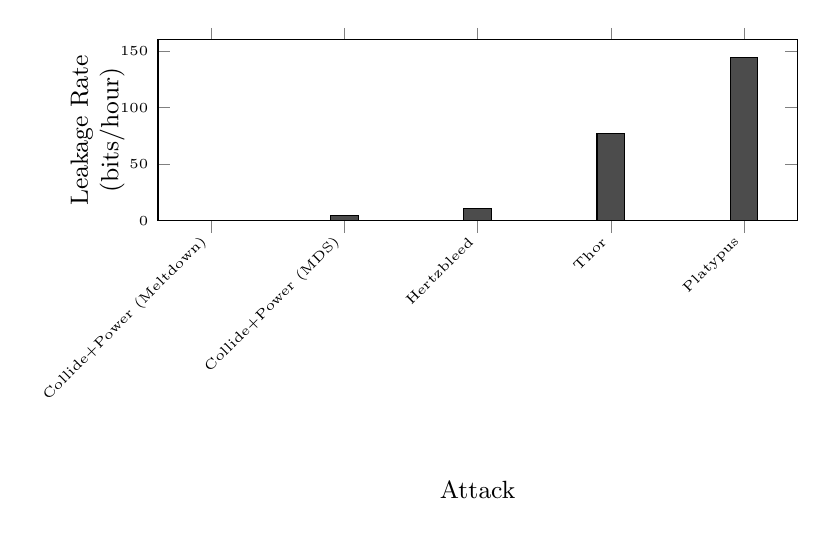
\begin{tikzpicture}
    \begin{axis}[
        ybar,
        symbolic x coords={Collide+Power (Meltdown), Collide+Power (MDS), Hertzbleed, Thor, Platypus},
        xtick=data,
        width=\linewidth*0.8,
        height=\linewidth*0.32,
        xlabel={Attack},
        ylabel={Leakage Rate\\(bits/hour)},
        ymin=0,
        ymax=160,
        x tick label style={
            rotate=45, 
            anchor=east,
            font=\tiny 
        },
        y tick label style={
            font=\tiny 
        },
        bar width=10pt,
        xlabel style={yshift=-0.7cm, font=\small},
        ylabel style={yshift=-0.3cm, align=center, font=\small},
    ]
        \addplot[
        color=black, 
        fill=black!70] coordinates {
            (Collide+Power (Meltdown), 0.136)
            (Collide+Power (MDS), 4.82)
            (Hertzbleed, 10.5)
            (Thor, 76.8)
            (Platypus, 144.7)
        };
    \end{axis}
\end{tikzpicture}
    \caption{\textsc{Thor} leakage rate comparison.}
    \label{fig:thorleakage}
\end{figure}
%
\subsection{Counter-measurement}
\begin{comment}
\textsc{Thor} relies only on precise \textit{timing} measurements. Therefore, it cannot be mitigated by defenses that alter the classification output of NNs, such as adding noise or rounding confidence scores \cite{Fredrikson2015ModelInversion}. 
Trusted Execution Environment (TEE)-based defenses, such as those performing non-linear computations inside the TEE while offloading linear computations to untrusted sources \cite{tramèr2019slalomfastverifiableprivate}, are also inadequate since we confirmed that the value dependencies of Intel AMX timing that \textsc{Thor} relies on are unaffected by TEE environments like Intel SGX. 
AI workloads demand high speed and efficiency, prompting AI libraries to prioritize performance optimizations. As a result, known constant-time programming techniques are often unsuitable as a defense. For example, masking can help protect weights from leaking but introduces extra computational overhead, increasing both power consumption and execution time.
\end{comment}
\textsc{Thor} relies only on precise \textit{timing} measurements. Thus, it cannot be mitigated by defenses that alter NN classification outputs, such as adding noise or rounding confidence scores \cite{Fredrikson2015ModelInversion}. Trusted Execution Environment (TEE)-based defenses, like those performing non-linear computations inside the TEE while offloading linear computations to untrusted sources \cite{tramèr2019slalomfastverifiableprivate}, are also inadequate, as the value dependencies of Intel AMX timing that \textsc{Thor} relies on are unaffected by TEE environments like Intel SGX. AI workloads demand high speed and efficiency, prompting AI libraries to prioritize performance optimizations. As a result, known constant-time programming techniques are often unsuitable as a defense. For example, masking can help protect weights from leaking but introduces extra computational overhead, increasing both power consumption and execution time.

A more effective strategy involves introducing response randomness by delaying execution, which disrupts the timing signals relied upon by \textsc{Thor}. However, this approach adds latency to AI applications. Limiting the query rate of the model 
could also slow these attacks, but at the cost of reducing system responsiveness.
Extending detection mechanisms, 
to identify malicious patterns in power and performance characteristics offers a promising defense against \textsc{Thor}.
Lastly, employing homomorphic encryption 
could provide robust protection but comes with substantial computational overhead and performance costs, making it less practical for high-speed AI applications.


%\subsection{Power \& Performance Overhead}
% In an experiment, we measured the time to execute a single AMX multiplication instruction while varying the intervals between consecutive executions. By adjusting the length of these intervals, we identified five distinct execution times, classifying them into performance states. The shortest execution time with the lowest intervals was labeled as the "Warm State," while the longer execution times with higher intervals were classified as "Cold States." 
One mitigation which can be applied through a micro-code update or a software patch is to keep the AMX unit moderately in the Warm State at all times or at least during Intel SGX execution to protect TEEs computation against \textsc{Thor}.
%
This approach is effective because we observed that timing differences dependent on zero values are only significantly measurable when the Intel AMX is in a Cold State. Warm and Cold States introduced here come from an interesting observation in which 
%In an experiment, 
we measured the time to execute a single AMX multiplication instruction while varying the intervals between consecutive executions. By adjusting the length of these intervals, we identified five distinct execution times, classifying them into performance states. The shortest execution time with the lowest intervals was labeled as the Warm State, while the longer execution times with higher intervals were classified as Cold States.  These performance states are shown in Figure~\ref{fig:Performance_Stages}.
However, this mitigation comes with trade-offs in power management and execution speed, as system power limits could be more easily reached, leading to unnecessary throttling of the AMX unit. We measured the power overhead of such defense for \textsc{Thor} and found that depending on the cold vs. warm stage,  the overhead ranges from 2.59\% to 12.33\%. Although this secure design requires more power consumption, it is faster as it keeps the Intel AMX in the highest performance state at all time; this is in contrary to other secure designs for different microarchitectural attacks which almost always incurred a high performance overhead. 
%\textcolor{red}{Todo  quantitatively calculate the AMX latency in warm state over cold state and add numbers here saying how much faster approx.  }

%Although the secure design requires more power consumption, it could be faster in scenarios such as workloads with infrequent multiplications.
\begin{figure}
    \centering
    \begin{tikzpicture}
        \begin{axis}[
            xmin=100, xmax=1000000000,
            ymin=10, ymax=100000,
            xlabel={Interval Delay (Cycle)},
            ylabel={Multiplication Execution\\Time (Cycle)},
            xmode=log, 
            ymode=log,
            log basis x=10, 
            log basis y=10,
            grid=both,
            major grid style={line width=0pt,draw=white!50},
            minor grid style={line width=0pt,draw=white!20},
            font=\scriptsize,
            ylabel style={yshift=0pt, align=center}, 
            width=\linewidth*1,
            height=\linewidth*0.45,
        ]
            \addplot[darkgray, thick] table {Diagrams/Data/warmup.txt};
        \end{axis}
        
        \draw[->, black, thick] (2.1,0.45) -- (1.1,0.45) node[midway, above] {\scriptsize Warm State};
         \node[gray, thick] at (1.05,1.3) {\scriptsize Cold State 1};
         \node[gray, thick] at (2.8,1.7) {\scriptsize Cold State 2};
         \node[gray, thick] at (4.9,1.85) {\scriptsize Cold State 3};
         \node[gray, thick] at (6.4,2.15) {\scriptsize Cold State 4};
         
    \end{tikzpicture}
    \caption{  Performance States of
TMUL and the Secure Recommended Intel AMX Operational State (Warm).}
    \label{fig:Performance_Stages}
\end{figure}

Thus, future research must prioritize the development of effective mechanisms to mitigate the proposed threat vector introduced by AMX and similar technologies while addressing the secure design's performance and power consumption. 

% \section{Conclusion}
% \section*{Conclusion}
This paper aims to enhance our understanding of the computational complexity of computing various Shapley value variants. We found that for various ML models --- including decision trees, regression tree ensembles, weighted automata, and linear regression --- both local and global interventional and baseline SHAP can be computed in polynomial time under HMM modeled distributions. This extends popular algorithms, such as TreeSHAP, beyond their empirical distributional scope. We also establish strict complexity gaps between the various SHAP variants (baseline, interventional, and conditional) and prove the intractability of computing SHAP for tree ensembles and neural networks in simplified scenarios. Overall, we present SHAP as a versatile framework whose complexity depends on four key factors: \begin{inparaenum}[(i)] \item model type, \item SHAP variant, \item distribution modeling approach, \item and local vs. global explanations\end{inparaenum}. We believe this perspective provides deeper insight into the computational complexity of SHAP, paving the way for future work.




%We believe that our framework provides a more intricate understanding of SHAP computation complexity across different models, distributions, and variants, paving the way for further research.

Our work opens promising directions for future research. First, expanding our computational analysis to other SHAP-related metrics, such as asymmetric SHAP~\citep{frye20} and SAGE~\citep{covert2020understanding}, would be valuable. Additionally, we aim to explore more expressive distribution classes and relaxed assumptions beyond those in Section \ref{sec:tractable} while maintaining tractable SHAP computation. Finally, when exact computation is intractable (Section \ref{sec:intractable}), investigating the approximability of SHAP metrics through approximation and parameterized complexity theory~\citep{downey2012parameterized} is an important direction.

%Our work opens several promising avenues for future research on the computational properties of explainable AI methods, with a particular focus on SHAP. First, it would be interesting to broaden the computational analysis conducted in this work to include other popular SHAP-related metrics in the literature, such as asymmetric SHAP \cite{frye20} and SAGE \cite{covert2020understanding}. Also, in the future, we aim to explore more expressive distribution classes and relaxed distributional assumptions—extending beyond those examined in Section \ref{sec:tractable} —that still yield tractable SHAP computation. Finally, when exact computation proves intractable (Section \ref{sec:intractable}), it is worthwhile to theoretically investigate the question of the approximability of computing the SHAP metrics across various configurations, through the lens of approximation and parametrized complexity theory \cite{arora2009computational}.

%This paper aims to deepen our understanding of the computational complexity involved in obtaining different Shapley value variants. We found that for a variety of ML models, including decision trees, tree ensembles for regression, weighted automata, and linear regression models — computing both local and global interventional and baseline SHAP can be done in polynomial time when distributions are modeled by HMMs. This extends the distributional scope of popular algorithms like TreeSHAP, which is limited to empirical distributions. Additionally, we demonstrate a strict complexity gap between SHAP variants, showing that interventional and baseline SHAP can be strictly easier to compute than conditional SHAP. Despite these positive results, we uncovered intractability for various SHAP variants in neural networks and tree ensembles. Finally, we provided generalized complexity relations across SHAP variants. We believe that our framework offers a deeper understanding of the complexity involved in computing SHAP across various variants, models, distributions, as well as in both local and global computations, laying the groundwork for future research.

%\section*{Acknowledgments}
%\section{Acknowledgments}
We would like to thank Kostis Kaffes, Tanvir Ahmed Khan, and Yuhong Zhong for their feedback.
We also thank the CloudLab team for their help in supporting our experiments.
This work was supported by IBM, and NSF awards CNS-2143868 and CNS-2106530.
Tal Zussman was supported by NSF award DGE-2036197.
Ioannis Zarkadas is an Onassis Foundation scholar.


%{\appendix[Proof of the XYZ Equation]
%Hi
%}

%\section{Related works}
Implicit Neural Representations are designed to learn continuous representations of target functions by taking advantages of the approximation power of neural networks.
%
Their inherent continuous property can beneficial in many cases like video compression~\citep{chen2021nerv,strumpler2022implicit}, 3D modeling~\citep{park2019deepsdf,atzmon2020sal,9010266,gropp2020implicit,sitzmann2019scene} and volume rendering~\citep{pumarola2021d, barron2021mip,martin2021nerf,barron2023zip}.
%
However, simply employing MLPs may result in spectral bias, where oversmoothed outputs are generated due to the inherent tendency of MLPs to prioritize learning low-frequency components first. Consequently, many studies have focused on these drawbacks and explored various methods to address this issue.
%
The most straightforward way to address this issue is by projecting the coordinates into the higher dimension~\citep{tancik2020fourier, wang2021spline}.
%
However, these methods can lead to noisy outputs if there is a mismatch in the embeddings variance.
%
To address this, \citet{landgraf2022pins} propose dividing the Random Fourier Features into multiple levels of detail, allowing the MLPs to disregard unnecessary high-frequency components. Another type of approach to mitigating the spectral bias introduced by the ReLU activation function, as proposed by \citet{sitzmann2020implicit}, \citet{ramasinghe2022beyond}, \citet{saragadam2023wire}, and \citet{shenouda2024relus}, is to modify the activation function itself by using alternatives such as the Sine function, Wavelets, or a combination of ReLU with other functions. There are also efforts to modify network structures to mitigate spectral bias~\citep{mujkanovic2024neural}. 
%
\citet{lindell2022bacon} introduce a network design that treats MLPs as filters applied to the input of the next layer, known as Multiplicative Filter Networks (MFNs). 
%
Additionally, based on the discrete nature of signals like images and videos, grid-based approaches (e.g., Grid Tangent Kernel~\citep{zhao2024grounding}, DINER~\citep{xie2023diner}, and Fourier Filter Bank~\citep{wu2023neural}) have been proposed to address spectral bias, as the grid property allows for sharp changes in features, which facilitates learning fine details.
Even though, there are some prior works trying to solve the inherent problems of Fourier features embeddings ~\citep{landgraf2022pins, yuce2022structured, hertz2021sape, saratchandran2024sampling}, limited research has addressed both the underlying causes of high-frequency noise and provides a non-heuristic solution even if these embeddings are widely employed into many downstream tasks.
%\section{Background}\label{sec:background}

%\section{Mobile Networks Powered by \glspl{LLM}}
\label{sec:LLM_enabled_MNs}
\begin{figure*}[t!]
\centering
\includegraphics[width=.99\textwidth]{Fig1.eps}
    \caption{Possible architectural designs for integrated \gls{LLM} and \gls{MNO} ecosystem.}
    \label{fig:LLM_possible_architectures}
\end{figure*}
The historical data of the \gls{MNO}, archived over years of expertise, constitutes a solid foundation for training the \gls{LLM} using structured and unstructured multi-modal inputs (as illustrated in Fig.~\ref{fig:LLM_possible_architectures}a) such as user intents, network logs, alarm descriptions, trouble tickets, \gls{PCAP} files (e.g. from Wireshark or tcpdump), dashboard screenshots, audio recordings (e.g. from \gls{IVR} systems), video feeds (e.g. from infrastructure surveillance), and \gls{NWDAF} analytics. To this end, a separate collection framework aggregates data from various sources into a centralized repository, and extracts most informative features such as warnings, error codes, timestamps, and user/gNB/session/bearer/\gls{QoS} flow/slice IDs. The extracted features are then converted into unified embeddings that are combined into a common vector space with suitable metadata (e.g. to differentiate data formats). The resulting vector store is used to fine-tune the \gls{LLM} to deeply internalize \gls{MNO}-specific knowledge \cite{Bariah2023understanding}. This allows the \gls{LLM} to learn patterns, sequences, and deviations that correlate with normal or faulty network operations. This is made possible using a timestamp-based cross-referencing to link different entries from several data sources, allowing detailed description and context for each flagged event as well as the resolution workflow for the spotted anomalies.

In live mobile networks, fresh multi-modal data is continuously fed into the \gls{LLM}, either uploaded in batches or streamed in real-time. The \gls{LLM} analyzes this data and identifies potential anomalous behaviors in light of its accumulated learning. In case of new anomalies not covered during the fine-tuning stage, the \gls{LLM} can rely on clustering techniques to group similar patterns and flag outliers as suspected behaviors. The \gls{LLM} is also capable of using \gls{RAG}-enabled external knowledge databases such as \gls{3GPP} documents \cite{Said2024instruct}, \gls{IEEE} standards, \gls{IETF} RFCs and vendors documentation \cite{soman2023observations} to compare the actual network behavior with the expected one to identify misconfigurations and spot unusual trends in protocols and communication flows. Well-crafted prompts, on the other hand, can guide the \gls{LLM} responses to provide focused solutions. Paradigms such as the \gls{CoT} reasoning can be used to break down the \gls{LLM} insights into a series of simplified and actionable sub-tasks. It can be extended by the \gls{ToT} technique to explore different reasoning paths and identify the most optimal solution. The \gls{LLM} can naturally produce stepwise reasoning if datasets used for fine-tuning contain \gls{CoT} and \gls{ToT} examples, or through creative prompting \cite{Zhou2024survey}. In parallel, \gls{NOC} engineers can intervene to confirm, guide or reject the \gls{LLM} findings, if needed, e.g. using its intuitive conversational interface. Through continuous self-learning, the \gls{LLM} will dynamically adapt to evolving network conditions, optimizing its performance over time \cite{Chaparadza2023optimization}.

%For instance, when a network experiences latency issues, the \gls{LLM} seamlessly analyze multi-modal information from diverse origins to identify the root cause, e.g. overloaded \gls{UPF} due to insufficient capacity, and then suggest a solution, e.g. step-by-step instructions including suitable code scripts for the involved \glspl{NF} to autonomously reroute traffic or modify policies. Conventional 5G networks can only alert about anomalies using suitable \gls{NWDAF} analytics that track the violated thresholds and notify the \gls{OAM} center to display the details on complex dashboards.

By incorporating \glspl{LLM} (e.g. as \glspl{NF}) into upcoming 6G networks, expected to be designed with \gls{SbD} principles \cite{Khaloopour2024Resilience}, \glspl{LLM} will naturally inherit the same built-in security safeguards rather than adding them as an afterthought. This design-driven approach focuses on proactive threat management, end-to-end encryption, authentication, network slicing isolation, \gls{AI}-driven threat detection with automated reactions, and stateless designs, fostering a resilient \gls{LLM}.
%The design-driven security in 5G and upcoming 6G networks ensures that security is natively integrated at every layer of the architecture rather than added as an afterthought. This approach focuses on proactive threat management, end-to-end encryption, authentication, network slicing, and \gls{AI}-driven threat detection and automated reactions to counter evolving cyber threats.



\end{spacing}

\begin{spacing}{0.95}
    
%\vspace{-1em}
\bibliographystyle{IEEEtranS}
\bibliography{refs}
\end{spacing}
\vfill
%


% \begin{figure}[!t]
%     \centering
%    \includegraphics[width=\linewidth] {images/AMXarch_new_v1.pdf} 
%     \caption{Intel AMX Architecture Overview}
%     \label{fig:AMX-arch}
% \end{figure}

% \subsection{Intel AMX Architecture and Instructions.}
% Intel AMX is an integrated accelerator introduced with the 4th Gen Intel Xeon Scalable processors, specifically engineered to boost the efficiency of matrix computations. %Figure~\ref{fig:AMX-arch} illustrates the Intel AMX architecture.

% AMX introduces a new set of registers and instructions. The registers in Intel AMX are known as Tiles, a new concept in Intel CPUs that provide a matrix of data registers, as opposed to the traditional vector registers seen in previous SIMD architectures like AVX-512. AMX includes 8 Tile registers, each capable of holding up to 16 rows with 64 bytes per row, amounting to a total of 1 KB per Tile. The number of rows and the number of bytes per row can be adjusted using the LDTILECFG instruction, and this configuration information is stored as metadata in a control register known as TILECFG. Once this configuration is set, AMX instructions such as load, store, and matrix multiplication will operate according to the specified dimensions for each Tile. Intel AMX instructions are synchronized with the Intel Architecture host (IA host) instruction stream, and the Tile loads and stores are coherent with the host memory \cite{Intel_Arc_Ins_Set_Extensions}.

% Tile Matrix Multiply unit (TMUL) serves as the accelerator engine for executing multiplication calculations. When using full-size Tile operands, the latency of the multiplication instruction is 52 cycles, while pipelining allows for a throughput of 16 cycles. Intel AMX supports two data types: BF16 and INT8. Consequently, it can perform 512 multiplications and 512 additions per cycle for BF16 and 1024 multiplications and 1024 additions per cycle for INT8 \cite{IntelOptRefManual}. 

% \begin{comment}
% AMX instructions utilize port 5 as their dedicated execution port. When two hyper-threads are active within a core, they compete for the same resources to execute AMX instructions.
% \end{comment}

\section{Reverse Engineering}
In this section, we share our findings on Intel AMX obtained through reverse engineering. In our investigations, we utilized a server running Red Hat Enterprise Linux release 9.3 (Plow), equipped with Linux kernel version 5.14. The server is powered by two Intel(R) Xeon(R) Gold 5420+ CPUs. 
We did not disable any hardware features or mitigations.

\textbf{Performance States Characterization.} 
In an experiment, we measured how long it takes to execute a single AMX multiplication instruction while varying the intervals between consecutive executions. To simulate the conditions of a typical program, we added non-AMX instructions during these intervals. By changing the length of these intervals, we observed five distinct execution times for the AMX multiplication instruction. We classified these into performance states, with the shortest execution time labeled as the "Warm State." The longer execution times are referred to as "Cold States," specifically Cold State 1 (the second shortest), Cold State 2, Cold State 3, and Cold State 4 (the longest).  Figure \ref{fig:Performance_Stages} visually represents these performance states. 

%\begin{figure}[!hbp]
%\centering\includegraphics[width=0.4\textwidth]{images/sleepstages_new_v2.pdf}
%\caption{Illustration of the Five Distinct Performance States of TMUL.}
%\label{fig:Performance_Stages}
%\end{figure}
%{\color{blue} Change the figure: bias, change the ylabel, and States }

\begin{figure}
    \centering
    \begin{tikzpicture}
        \begin{axis}[
            xmin=100, xmax=1000000000,
            ymin=10, ymax=100000,
            xlabel={Interval Delay (Cycle)},
            ylabel={Multiplication Execution\\Time (Cycle)},
            xmode=log, 
            ymode=log,
            log basis x=10, 
            log basis y=10,
            grid=both,
            major grid style={line width=0pt,draw=white!50},
            minor grid style={line width=0pt,draw=white!20},
            font=\scriptsize,
            ylabel style={yshift=0pt, align=center}, 
            width=\linewidth*1,
            height=\linewidth*0.45,
        ]
            \addplot[darkgray, thick] table {Diagrams/Data/warmup.txt};
        \end{axis}
        
        \draw[->, black, thick] (2.1,0.45) -- (1.1,0.45) node[midway, above] {\scriptsize Warm State};
         \node[gray, thick] at (1.05,1.3) {\scriptsize Cold State 1};
         \node[gray, thick] at (2.8,1.7) {\scriptsize Cold State 2};
         \node[gray, thick] at (4.9,1.85) {\scriptsize Cold State 3};
         \node[gray, thick] at (6.4,2.15) {\scriptsize Cold State 4};
         
    \end{tikzpicture}
    \caption{llustration of the Five Distinct Performance States of
TMUL.}
    \label{fig:Performance_Stages}
\end{figure}

%\begin{spacing}{1}
% \begin{lstlisting}
% for(int i = 0; i < ITERS;i++) {
%   Time = __rdtscp();// Timer
%   for (int k = 0; k < i; k++)// Delay
%      junk = junk + k;
%   cooldown_delay[i] = __rdtscp() - Time; 
%   Time =  __rdtscp()
%   AMX_INSTRUCTION();//e.g_tile_dpbssd(0, 1, 2)
%   execution_time[i] = __rdtscp() - Time; }
% \end{lstlisting}
%\end{spacing}

\textbf{Impact of CPU Frequency on Performance States.} 
In a supplementary experiment, we investigated how changing the CPU frequency, using the "cpufreq" feature, affects the execution time of the previously identified performance states. For this study, we fixed the CPU frequency at various levels and measured the execution times for each performance state without allowing frequency scaling to adjust it dynamically. 

The results are plotted in Figure \ref{fig:Execution_time_vs_Freq}, where each data point represents a specific CPU frequency setting. Execution time was recorded using the `rdtscp` instruction, which operates with a 2 GHz clock frequency reference. We examined frequencies ranging from 800 MHz to 2 GHz in increments of 100 MHz.

Our findings indicate that the execution time of the AMX multiplication instruction in all Cold States is invariant with respect to changes in the current CPU frequency. In contrast, the Warm State execution time is directly proportional to the current CPU frequency.

%\begin{figure}[!hbp]
%\centering\includegraphics[width=0.4\textwidth]{images/Execution_time_vs_Freq.pdf}
%\caption{Execution Time of AMX Multiplication Across Performance States at Varying CPU Frequencies}
%\label{fig:Execution_time_vs_Freq}
%\end{figure}
%{\color{blue} Put Execution\_time\_vs\_Freq figure here}


\begin{figure}[t!]
\centering
\begin{tikzpicture}
    \begin{axis}[
        xlabel={CPU Frequency (MHz)},
        ylabel={Execution time (RDTSCP cycle)},
        legend pos=outer north east,
        font=\scriptsize,
        xlabel style={yshift=0pt},
        ylabel style={yshift=0pt},
        width=\linewidth*0.8,
        height=\linewidth*0.45,
        ymode=log,
        log basis y=10,
        legend style={
                legend columns=1, 
                at={(1.02,0.5)}, 
                anchor=west,   
                font=\tiny,
            },
    ]
    
    \addplot[
        thick,
        mark=diamond,
        line width=1.5pt,
        mark size=3,
        color=darkgray
    ] table {Diagrams/Data/freq4.txt};
    \addlegendentry{Cold State 4};

    \addplot[
        thick,
        mark=x,
        line width=1.5pt,
        mark size=3,
        color=darkgray
    ] table {Diagrams/Data/freq3.txt};
    \addlegendentry{Cold State 3};
 
    \addplot[
        thick,
        line width=1.5pt,
        mark=triangle,
        mark size=2,
        color=darkgray
    ] table {Diagrams/Data/freq2.txt};
    \addlegendentry{Cold State 2};

    \addplot[
        thick,
        mark=star,
        line width=1.5pt,
        mark size=3,
        color=darkgray
    ] table {Diagrams/Data/freq1.txt};
    \addlegendentry{Cold State 1};
   
    \addplot[
        thick,
        line width=1.5pt,
        mark=o,
        mark size=2,
        color=red
    ] table {Diagrams/Data/freq0.txt};
    \addlegendentry{Warm State};



    \end{axis}
\end{tikzpicture}
\caption{Execution Time of AMX Multiplication Across Performance States at Varying CPU Frequencies}
\label{fig:Execution_time_vs_Freq}
\end{figure}

\textbf{Transition Behavior of AMX Frequency to CPU Frequency in Warm State.}
Based on the results presented in Figure \ref{fig:Performance_Stages}, the execution of the TMUL multiplication instruction occurs in Cold State 4 (the longest execution time) when either the operation is performed for the first time or follows a period of inactivity exceeding approximately 20 ms. If subsequent AMX multiplication instructions follow closely, all will operate in the Warm State, which is common in programs with extensive matrix multiplications.

We further examined the execution time in the Warm State immediately after entry, over a fixed duration, across different CPU frequencies. Our observations revealed that the AMX multiplication execution time undergoes a transition period before stabilizing. Closer analysis shows that these variations are related to the AMX's internal frequency adjustments. During this transition period, AMX adjusts its frequency from a lower value towards the current CPU frequency, temporarily using intermediate frequencies.

Figure \ref{fig:Freq_transition} illustrates how the AMX frequency adjusts to align with the CPU frequency. When the CPU frequency is set to 1.2 GHz, the AMX frequency initially ramps up, briefly stabilizes at 1 GHz, and eventually reaches the target frequency of 1.2 GHz. Similarly, when the CPU frequency is fixed at 2 GHz, the AMX frequency transitions through intermediate stages, operating at 1 GHz and 1.3 GHz before stabilizing at 2 GHz.

These findings demonstrate that Intel AMX includes a frequency management unit that controls the operating frequency of the TMUL accelerator. This unit can potentially access or create frequencies that differ from the CPU frequency.

%\begin{figure}[!hbp]
%\centering\includegraphics[width=0.4\textwidth]{images/Freq_transition.pdf}
%\caption{Illustration of AMX Frequency Adjustment During Transition Periods: (a) shows the transition to a 1.2 GHz CPU frequency, with intermediate operation at 1 GHz; (b) demonstrates the adjustment to a 2 GHz CPU frequency, passing through 1 GHz and 1.3 GHz stages.}
%\label{fig:Freq_transition}
%\end{figure}
%{\color{blue} Put Freq\_transition figure here}

\begin{figure}[h!]
\centering
\begin{tikzpicture}
    \begin{axis}[
        xlabel={Number of Instructions},
        ylabel={Execution Time (RDTSCP cycle)},
        legend pos=outer north east,
        font=\scriptsize,
        xlabel style={yshift=5pt},
        ylabel style={yshift=-15pt},
        width=\linewidth*1,
        height=\linewidth*0.45,
        xmin= -0.1,xmax=40000,
        legend style={
                legend columns=-1,
                at={(0.5,1.16)},
                anchor=north, 
                font=\tiny,
                /tikz/column 2/.style={column sep=5pt}, 
            },
    ]
    
    \addplot[
        line width=0.8pt,
        color=black,
    ] table {Diagrams/Data/1400MHz.txt};
    \addlegendentry{1.2 GHz
CPU frequency};


    \addplot[
        line width=0.8pt,
        color=lightgray,
    ] table {Diagrams/Data/2000MHz.txt};
    \addlegendentry{2 GHz
CPU frequency};

    \end{axis}
    
    \node[darkgray, thick] at (2.7,1.57) {\scriptsize 1 GHz};
    \node[darkgray, thick] at (5.7,1.175) {\scriptsize 1.2 GHz};
    \node[darkgray, thick] at (2.5,1.01) {\scriptsize 1.3 GHz};
    \node[darkgray, thick] at (5.5,0.37) {\scriptsize 2 GHz};
\end{tikzpicture}
\caption{Illustration of AMX Frequency Adjustment During Transition Periods: The black graph depicts the transition to a 1.2 GHz CPU frequency, with intermediate operation at 1 GHz; The gray graph demonstrates the adjustment to a 2 GHz CPU frequency, passing through 1 GHz and 1.3 GHz stages.}
\label{fig:Freq_transition}
\end{figure}

\textbf{Impact of Operand Sparsity on TMUL Transition in Warm State.}
In our investigation of the TMUL execution time transition in the Warm State, we discovered an interesting effect involving zero values in the Tile operands during multiplication. By varying the number of zero values in the operands, we observed that increasing the number of zeros accelerates the transition period. This effect is illustrated in Figure \ref{fig:Effect_of_zeros_on_transition}, which presents three graphs depicting operand sparsity levels: 100\% sparsity, 50\% sparsity, and 0\% sparsity. In Figure \ref{fig:Effect_of_zeros_on_transition}, with the CPU frequency fixed at 2 GHz, the results indicate that higher operand sparsity in the Tile operands leads to faster convergence of the TMUL frequency to the CPU frequency.

%\begin{figure}[!hbp]
%\centering\includegraphics[width=0.4\textwidth]{images/Effect_of_zeros_on_transition.pdf}
%\caption{Impact of Operand Sparsity on the Transition Period of TMUL Frequency: The graphs depict the transition behavior with 100\%, 50\%, and 0\% sparsity levels in the Tile operands, showing faster convergence to the CPU frequency with increased sparsity.}
%\label{fig:Effect_of_zeros_on_transition}
%\end{figure}
%{\color{blue} Put Freq\_transition figure here}

\begin{figure}[h!]
\centering
\begin{tikzpicture}
    \begin{axis}[
        xlabel={Number of Instructions},
        ylabel={Execution Time (RDTSCP cycle)},
        legend pos=outer north east,
        font=\scriptsize,
        xlabel style={yshift=5pt},
        ylabel style={yshift=-15pt},
        width=\linewidth*1,
        height=\linewidth*0.48,
        xmin= -0.1,xmax=40000,
        legend style={
                legend columns=-1,
                at={(0.5,1.16)},
                anchor=north, 
                font=\tiny,
                /tikz/column 2/.style={column sep=5pt}, 
            },
    ]
    
    \addplot[
        line width=0.8pt,
        color=black,
    ] table {Diagrams/Data/2000_0Perc.txt};
    \addlegendentry{0\% Sparcity};


    \addplot[
        line width=0.8pt,
        color=lightgray,
    ] table {Diagrams/Data/2000_50Perc.txt};
    \addlegendentry{50\% Sparcity};


    \addplot[
        line width=0.8pt,
        color=gray,
    ] table {Diagrams/Data/2000_100Perc.txt};
    \addlegendentry{100\% Sparcity};

    \end{axis}
    
    \node[darkgray, thick] at (1.2,0.57) {\scriptsize 1.8 GHz};
    \node[darkgray, thick] at (1.9,1.95) {\scriptsize 1 GHz};
    \node[darkgray, thick] at (2,1.23) {\scriptsize 1.3 GHz};
    \node[darkgray, thick] at (5.5,0.4) {\scriptsize 2 GHz};
\end{tikzpicture}
\caption{Impact of Operand Sparsity on the Transition Period of TMUL Frequency: The graphs depict the transition behavior with 100\%, 50\%, and 0\% sparsity levels in the Tile operands, showing faster convergence to the CPU frequency with increased sparsity.}
\label{fig:Effect_of_zeros_on_transition}
\end{figure}

Consequently, the execution time of a program utilizing AMX multiplications is closely associated with the sparsity of its input operands. In Figure \ref{fig:Cumulative_execution_time}, we demonstrate this relationship by executing two test programs with 100 and 1000 AMX multiplications, each with varying Tile operand sparsity levels (0\%, 50\%, and 100\%). To construct the histogram, each scenario was executed 1,000 times. Our results reveal that varying levels of sparsity significantly impact the cumulative execution time of AMX multiplications, with increased sparsity leading to faster program execution.

This discovery uncovers a new value-dependent timing side channel that reveals the sparsity of Tile operands in Intel AMX.

% \begin{figure}[htbp!]
%     \centering
%     \begin{tikzpicture}
%         \begin{axis}[
%             font=\scriptsize,
%             width=\linewidth*0.95,
%             height=\linewidth*0.35,
%             bar width=50,
%             xmin=21800, xmax=24650,
%             xlabel={Execution time (cycle)},
%             ybar,
%             ylabel={Frequency},
%             ylabel style={yshift=-15pt},
%             ymin=0, ymax=0.006,
%             legend style={
%                 at={(0.5,1)}, 
%                 anchor=north, 
%                 legend columns=-1,
%                 font=\scriptsize,
%                 /tikz/column 2/.style={column sep=5pt}, 
%                 fill=none,
%                 draw=none
%             },
%             legend image code/.code={\draw[fill=#1,draw=none] (0cm,-0.1cm) rectangle (0.25cm,0.1cm);},
%             legend entries={100\% sparsity, 50\% sparsity, 0\% sparsity}
%         ]
%             \addplot+[hist={density, bins=50}, fill=lightgray, draw=none] table[y index=0] {Diagrams/Data/100-0.txt};
%             \addplot+[hist={density, bins=50}, fill=black, draw=none] table[y index=0] {Diagrams/Data/100-half.txt};
%             \addplot+[hist={density, bins=50}, fill=gray, draw=none] table[y index=0] {Diagrams/Data/100-1.txt};
%         \end{axis}
%         \node[anchor=south east] at (rel axis cs:-0.05,1) {(a)};
%     \end{tikzpicture}
%     \begin{tikzpicture}
%         \begin{axis}[
%             font=\scriptsize,
%             width=\linewidth*0.95,
%             height=\linewidth*0.35,
%             bar width=50,
%             xmin=35500, xmax=56000,
%             xlabel={Execution time (cycle)},
%             ybar,
%             ylabel={Frequency},
%             ylabel style={yshift=-15pt},
%             ymin=0, ymax=0.0024,
%             legend style={
%                 at={(0.5,1)}, 
%                 anchor=north, 
%                 legend columns=-1,
%                 font=\scriptsize,
%                 /tikz/column 2/.style={column sep=5pt}, 
%                 fill=none,
%                 draw=none
%             },
%             legend image code/.code={\draw[fill=#1,draw=none] (0cm,-0.1cm) rectangle (0.25cm,0.1cm);},
%             legend entries={100\% sparsity, 50\% sparsity, 0\% sparsity}
%         ]
%             \addplot+[hist={density, bins=60}, fill=lightgray, draw=none] table[y index=0] {Diagrams/Data/1000-0.txt};
%             \addplot+[hist={density, bins=60}, fill=black, draw=none] table[y index=0] {Diagrams/Data/1000-half.txt};
%             \addplot+[hist={density, bins=60}, fill=gray, draw=none] table[y index=0] {Diagrams/Data/1000-1.txt};
%         \end{axis}
%         \node[anchor=south east] at (rel axis cs:-0.05,1) {(b)};
%     \end{tikzpicture}
%     \begin{comment}
%     \begin{tikzpicture}
%         \begin{axis}[
%             font=\scriptsize,
%             width=\linewidth*0.95,
%             height=\linewidth*0.5,
%             bar width=50,
%             xmin=170000, xmax=345000,
%             xlabel={Execution time (cycle)},
%             ybar,
%             ylabel={Frequency},
%             ylabel style={yshift=-15pt},
%             ymin=0, ymax=0.00022,
%             legend style={
%                 at={(0.5,1)}, 
%                 anchor=north, 
%                 legend columns=-1,
%                 font=\scriptsize,
%                 /tikz/column 2/.style={column sep=5pt}, 
%                 fill=none,
%                 draw=none
%             },
%             legend image code/.code={\draw[fill=#1,draw=none] (0cm,-0.1cm) rectangle (0.25cm,0.1cm);},
%             legend entries={100\% sparsity, 50\% sparsity, 0\% sparsity}
%         ]
%             \addplot+[hist={density, bins=60}, fill=lightgray, draw=none] table[y index=0] {Diagrams/Data/10000-0.txt};
%             \addplot+[hist={density, bins=60}, fill=black, draw=none] table[y index=0] {Diagrams/Data/10000-half.txt};
%             \addplot+[hist={density, bins=60}, fill=gray, draw=none] table[y index=0] {Diagrams/Data/10000-1.txt};
%         \end{axis}
%         \node[anchor=south east] at (rel axis cs:-0.05,1) {(c)};
%     \end{tikzpicture}
%     \end{comment}
% \begin{comment}
% \caption{Cumulative Execution Time of Programs with Varying Operand Sparsity: The histogram illustrates the effect of operand sparsity on program execution time, highlighting that higher sparsity levels result in quicker execution across different counts of AMX multiplications. Subfigures (a), (b), and (c) represent programs with 100, 1,000, and 10,000 AMX multiplications, respectively.}
% \end{comment}
% \caption{Cumulative Execution Time of Programs with Varying Operand Sparsity: The histogram illustrates the effect of operand sparsity on program execution time, highlighting that higher sparsity levels result in quicker execution across different counts of AMX multiplications. Subfigures (a) and (b) represent programs with 100 and 1,000 AMX multiplications, respectively.}
% \label{fig:Cumulative_execution_time}
% \end{figure}


%\begin{figure}[!htbp]
%\centerline{\includegraphics[width=0.35\textwidth]{images/new_pic.pdf}}
%\caption{Cumulative Execution Time of Programs with Varying Operand Sparsity: The %histogram illustrates the effect of operand sparsity on program execution time, %highlighting that higher sparsity levels result in quicker execution across %different counts of AMX multiplications. Subfigures (a), (b), and (c) represent %programs with 100, 1,000, and 10,000 AMX multiplications, respectively.}
%\label{fig:Cumulative_execution_time}
%\end{figure}

\begin{comment}
\textbf{Operand Patterns Influencing Data-Dependent Timing in AMX Multiplications.}
In this part, we describe specific operand patterns that can accelerate the TMUL frequency transition, thereby reducing cumulative execution time. As previously mentioned, Intel AMX supports both BF16 and Int8 operand types. 

For BF16 operands, we examined both normal values and special values, including zero, subnormal, NaN, and infinity. Consider an element \( x \) in the first Tile operand being multiplied by an element \( y \) in the second Tile operand. Our findings indicate that to expedite the frequency transition, at least one of the operands \( x \) or \( y \) should be zero or subnormal, while the other should be a normal value. In Intel AMX, subnormal values are treated as zeros, meaning that if an input is subnormal, it will be considered as zero. Additionally, if an output element falls into the subnormal range, AMX returns zero for that element. Table \ref{tab:BF16Pattern} lists all possible cases for BF16 operands, highlighting those patterns that facilitate quicker transitions.



\begin{table}[ht]
    \centering
    \resizebox{0.49\textwidth}{!}{%
    \begin{tabular}{|c|c|c|c|}
        \hline
        \backslashbox{Operand 1}{Operand 2} & Normal & Zero/Subnormal & NaN/Inf \\ \hline
        Normal & - & \ding{51} & - \\ \hline
        Zero/Subnormal & \ding{51} & \ding{51} & - \\ \hline
        NaN/Inf & - & - & - \\ \hline
    \end{tabular}
    }
    \caption{BF16 Operand Patterns in Intel AMX: Cases marked with \ding{51} indicate patterns that expedite the TMUL frequency adjustment.}
\label{tab:BF16Pattern}
\end{table}

For Int8 operands, the data-dependent pattern involves zero values in two consecutive Int8 entries within a row. Specifically, this occurs in the \(2k\) and \(2k + 1\) columns of the Tiles, where \(k\) ranges from 0 to \(C/2 - 1\), with \(C\) representing the number of bytes in each row of the Tile. Suppose element \( x(r_1,2i) \) and element \( x(r_1,2i+1) \) in the first Tile are multiplied by element \( y(r_2,2j) \) and element \( y(r_2,2j+1) \) in the second Tile, respectively. Table \ref{tab:Int8Pattern} highlights the combinations of these 4 values that lead to a faster frequency transition.

\begin{table}[ht]
    \centering
    \resizebox{0.47\textwidth}{!}{%
    \begin{tabular}{|c|c|c|c|c|}
        \hline
        \backslashbox{Operand 1}{Operand 2} & [Z, Z] & [Z, N] & [N, Z] & [N, N] \\ \hline
        {[}Z, Z{]} & \ding{51} & \ding{51} & \ding{51} & \ding{51} \\ \hline
        {[}Z, N{]} & \ding{51} & - & \ding{51} & - \\ \hline
        {[}N, Z{]} & \ding{51} & \ding{51} & - & - \\ \hline
        {[}N, N{]} & \ding{51} & - & - & - \\ \hline
    \end{tabular}
    }
    \caption{Int8 Operand Patterns: Entries marked with \ding{51} indicate patterns that accelerate TMUL frequency transition.\newline \small(Z = Zero, N = Non-zero)}
\label{tab:Int8Pattern}
\end{table}

Our results suggest the presence of a zero-skipping mechanism for both BF16 and Int8 operands. The Int8 results indicate that zero-skipping evaluates two bytes concurrently, which is likely due to the simultaneous processing of two Int8 multiplications in a specific pipeline stage within TMUL. Bypassing this pipeline stage necessitates checking both consecutive bytes. We hypothesize that bypassing these Tile element multiplications reduces AMX energy consumption, allowing the frequency management unit to increase TMUL frequency with fewer restrictions. Although the latency and throughput of AMX multiplications are fixed in terms of AMX cycles, they are influenced by operand sparsity when viewed in CPU cycles.

\end{comment}
%\section{Data Overvaluation Attack}
In this section, we first provide the \textit{data overvaluation} attack against the SV and then generalize it for other metrics.

\subsection{Data Overvaluation against the SV}
Although the SV fairly allocates data values to honest clients, strategic clients can manipulate their SVs by misreporting data subsets for model retraining.
As shown in Equation (\ref{eq:sv}), the SV $\sv_{i, j}$ enumerates all subsets $\datasubset$ of the grand dataset $\granddataset$; 
for each subset $\datasubset \subset \granddataset$, a model $\mathcal{A}(\datasubset)$ is retrained, and its utility $v(\datasubset)$ is evaluated for calculating $\sv_{i, j}$. 
Let $\stoi$ denote the set of data blocks in $\datasubset$ that belong to client $i$, $\stominusi$ denote the others data blocks in $\datasubset$, i.e., $\stominusi = \datasubset / \stoi$, and $\clientsins$ denote the set of clients who have at least one data block in $\datasubset$. 
Then, for each subset $\datasubset \subset \granddataset$ with $i \in \clientsins$, since $v(\datasubset)$ can also be expressed as $v(\stoi \cup \stominusi)$, client $i$ can vary $v(\datasubset)$ by misreporting $\stoi$, thereby manipulating their block-level SVs $\sv_{i, j}$.

Similarly, client $i$ can also manipulate their client-level SV $\sv_{i}$ by altering the model utility $v(\datasubset)$.
Specifically, the client-level SV $\sv_{i}=\sum_{j\in[M_i]}\sv_{i,j}$ can be written in the following form:
\begin{align*}
     &\sv_{i}(\granddataset, v) = \sum_{\datasubset\subseteq \granddataset} \betasv(\datasubset) \cdot v(\datasubset), \text{ where} \\
      & \betasv(\datasubset) \\
      \coloneqq &
   \begin{cases}
            \scriptstyle(|\stoi||\granddataset| - |D_{i}||\datasubset|) \cdot \frac{(|\datasubset |- 1)! (|\granddataset|-|\datasubset| - 1)!}{|\granddataset|!}, & \datasubset \subset \granddataset, \datasubset \neq \emptyset, \\
            |D_i|/ |\granddataset|, & \datasubset = \granddataset, \\
            - |D_i|/ |\granddataset|, & \datasubset = \emptyset.
   \end{cases}
\end{align*}
Because $\frac{\partial \sv_i}{\partial (v(\datasubset))} = \betasv(\datasubset)$, when $\betasv(\datasubset) > 0$, increasing $v(\datasubset)$ can enhance $\sv_{i}$; when $\betasv(\datasubset) < 0$, decreasing $v(\datasubset)$ improves $\sv_{i}$; when $\betasv(\datasubset) = 0$, changing $v(\datasubset)$ reduces $\sv_{i}$ has no effect on $\sv_{i}$.

\begin{algorithm}[t]
    \caption{Data Overvaluation against the SV}
    \label{alg:data_overvaluation}
\begin{algorithmic}[1]
   \STATE {\bfseries Input:} dataset $\granddataset$, grand model's utility $v(\granddataset)$
    \STATE {\bfseries Attacker:} client $i$
   \FOR{ each subset $\datasubset\subset \granddataset$}
        \IF{$i\in \clientsins$}
            \IF{$\betasv(\datasubset) > 0$}
                \STATE Client $i$: Positively augment $\stoi$ to obtain a reported dataset $\reportedstoi$.
            \ELSIF{$\betasv(\datasubset) < 0$}
                \STATE Client $i$: Negatively augment $\stoi$ to generate a reported dataset $\reportedstoi$.
            \ELSE
                \STATE Client $i$: Honestly use $\reportedstoi = \stoi$.
            \ENDIF
        \ENDIF
        \STATE Clients $\clientsins$: Use dataset $\reportedsubset=\cup_{i'\in \clientsins}  \widehat{D}^{\datasubset}_{i'}$ to train a model $\mathcal{A}(\reportedsubset)$.
        \STATE Server: Evaluate the model's utility $v(\reportedsubset)$.
   \ENDFOR
   \STATE Server: Calculate $\empiricalsv_{i,j}(\granddataset, v), \forall i, \forall j$ and return them.
   % \RETURN $\empiricalsv_{i,j}(\granddataset, v), \forall i$
\end{algorithmic}
\end{algorithm}

\textbf{Algorithm.}
Based on the above analysis, we propose Algorithm \ref{alg:data_overvaluation} to implement data overvaluation against the SV, considering a strategic client $i$ as an attacker.
Let $\reportedstoi$ denote the version of $\stoi$ reported by client $i$ and $\reportedstominusi$ denote the version of $\stominusi$ reported by the other clients for evaluating the model utility $v(\datasubset)$.
That means, instead of truthfully using dataset $\stoi$, client $i$ may untruthfully employ dataset $\reportedstoi \neq \stoi$ to increase the model utility from $v(\datasubset)$ to $v(\reportedsubset)$, where $\reportedsubset = \reportedstoi \cup \reportedstominusi$.
In Algorithm \ref{alg:data_overvaluation}, to compute the SV, we iterate over every subset $\datasubset \subset \granddataset$ and evaluate its corresponding model utility (Lines 3--18).
Note that the grand model's utility $v(\granddataset)$ is given as the algorithm's input, as the grand model $\mathcal{A}(\granddataset)$ has already been trained before data valuation. 
When a subset $\datasubset$ includes client $i$'s data blocks, if $\betasv(\datasubset)$ is nonzero, client $i$ has the incentive to manipulate $v(\datasubset)$; thus, in this case, client $i$ positively/negatively augments their dataset $\stoi$ to derive a new dataset $\reportedstoi$ (Lines 6 and 8), resulting in an enhanced/reduced utility $v(\reportedsubset)$ (Lines 13--14).
After evaluating all the model utilities, the server calculates client $i$'s \textit{empirical} block-level SVs as:
% \begin{align*}
%     &\sv_{i,j}(\granddataset, v \mid \forall \datasubset \subset \granddataset, \reportedstoi) \\
%     = & \sum_{\datasubset\subset \granddataset \setminus \set[D_{i,j}], i \in \clientsins} \weightsv(\datasubset) \big(v(\reportedsplustoi \cup \splustominusi)  - v(\reportedstoi \cup \stominusi)\big) \\
%     & + \sum_{\datasubset\subset \granddataset \setminus \set[D_{i,j}], i \notin \clientsins} \weightsv(\datasubset) \big(v(\reportedsplustoi \cup \splustominusi) -v(\datasubset)\big) \\
%     & + \frac{1}{|\granddataset|} \big(v(\granddataset)  - v(\widehat{D}^{\granddataset / \{D_{i,j}\}}_{i} \cup D^{\granddataset / \{D_{i,j}\}}_{-i})\big).
% \end{align*}

\begin{align*}
    \empiricalsv_{i,j}(\granddataset, v)\coloneqq & \sum_{\datasubset\subset \granddataset \setminus \set[D_{i,j}]} \weightsv(\datasubset) \big(v(\reportedsubset^{+})  - v(\reportedsubset)\big) \\
    & + \weightsv(\granddataset^{-}) \big(v(\granddataset)  - v(\widehat{D}_{\mathbb{N}}^{-})\big)
\end{align*}
where $\reportedsubset^{+}$ is the reported version of $\datasubset^{+}$, $\granddataset^{-} = \granddataset \setminus \{D_{i,j}\}$, and $\widehat{D}_{\mathbb{N}}^{-}$ is the reported version of $\granddataset^{-}$.
Consequently, client $i$ obtains their empirical client-level SV as:
% \begin{align*}
%     &\sv_{i}(\granddataset, v \mid \forall \datasubset \subset \granddataset, \reportedstoi) \\
%     = &\sum_{\datasubset\subseteq \granddataset, i\notin \clientsins} \betasv(\datasubset) \cdot v(\datasubset) \\
%     &+ \sum_{\datasubset\subseteq \granddataset, i \in \clientsins} \betasv(\datasubset) \cdot v(\reportedstoi \cup \stominusi), 
% \end{align*}
% which is guaranteed to be no less than the real SV $\sv_i(\granddataset, v)$ under certain circumstances as shown in Lemma \ref{lem:overvalued}.
\vspace{-3pt}
\begin{align*}
    \empiricalsv_{i}(\granddataset, v) = & \betasv(\granddataset) \cdot v(\granddataset) + \sum_{\datasubset\subset \granddataset} \betasv(\datasubset) \cdot v(\reportedsubset).
\end{align*}
If $\forall \datasubset \subset \granddataset$ with $\betasv(\datasubset) > 0$, we have $v(\reportedstoi \cup \reportedstominusi) \geq v(\stoi \cup \reportedstominusi)$, and $\forall \datasubset \subset \granddataset$ with $\betasv(\datasubset) < 0$, we have $v(\reportedstoi \cup \reportedstominusi) \leq v(\stoi \cup \reportedstominusi)$, then $\empiricalsv_{i}(\granddataset, v)$ is guaranteed to be no less than the empirical SV $\empiricalsv_i(\granddataset, v \mid \forall \datasubset \subset \granddataset, \reportedstoi =  \stoi)$ where client $i$ truthfully reports their data contributions $\reportedstoi = \stoi$, i.e.,
\begin{align*}
     &\empiricalsv_{i}(\granddataset, v \mid \forall \datasubset \subset \granddataset, \reportedstoi =  \stoi) \\
    = & \betasv(\granddataset) \cdot v(\granddataset) + \sum_{\datasubset\subset \granddataset} \betasv(\datasubset) \cdot v(\stoi \cup \reportedstominusi).
\end{align*}
This implies that client $i$ may increase its (empirical) client-level SV $\empiricalsv_{i}$ through a data overvaluation attack. 
Moreover, since the SV satisfies the EFF axiom, the total SV $\empiricalsv_{-i}$ of the other clients will decrease accordingly.

% \begin{lemma}
% \label{lem:overvalued}
%     When $v(\reportedstoi \cup \reportedstominusi) \geq v(\stoi \cup \reportedstominusi), \forall \datasubset \subset \granddataset, \betasv(\datasubset) > 0$ and $v(\reportedstoi \cup \reportedstominusi) \leq v(\stoi \cup \reportedstominusi), \forall \datasubset \subset \granddataset, \betasv(\datasubset) < 0$, we have $\empiricalsv_{i}(\granddataset, v) \geq \empiricalsv_{i}(\granddataset, v \mid \forall \datasubset \subset \granddataset, \reportedstoi =  \stoi)$ and $\empiricalsv_{-i}(\granddataset, v) \leq \empiricalsv_{-i}(\granddataset, v \mid \forall \datasubset \subset \granddataset, \reportedstoi =  \stoi)$.
% \end{lemma}


\subsection{Generalization}
In addition to the SV, we further generalize the data overvaluation attack to manipulate all linear data valuation metrics. 
% This generalization is highly fundamental because linearity is essential for fair and efficient data valuation and is satisfied by most mainstream valuation metrics.

\begin{lemma}
\label{lem:data_value_form}
    If a data valuation metric $\phi$ satisfies LIN, then for each client $i$, there exists $\beta_i: 2^{\granddataset} \rightarrow \mathbb{R}$ such that
    \begin{align*}
        \phi_{i}(\granddataset, v) \equiv \sum_{\datasubset \subseteq \granddataset} \beta_i(\datasubset) \cdot v(\datasubset).
    \end{align*}
\end{lemma}

Specifically, Lemma \ref{lem:data_value_form} indicates that any linear data value $\phi_i$ can be expressed as a weighted sum of model utilities $\{v(\datasubset)\}_{\datasubset\subseteq \granddataset}$. 
Consequently, similar to the case of the SV, for each subset $\datasubset \subset \granddataset$, and for each client $i\in\clientsins$, when $\beta_i(\datasubset)$ is positive (negative), they can increase (decrease) $v(\datasubset)$ to enhance their linear data value $\phi_i$.
However, unlike the SV, some data valuation metrics such as Beta Shapley and Banzhaf value do not satisfy EFF, meaning that an increase in $\phi_{i}$ does not necessarily lead to a decrease in $\phi_{-i}$.
As a result, client $i$ may not always receive a higher reward.
Therefore, when $\beta_{i}(\datasubset)$ is positive (negative), we should also ensure that $\beta_{-i}(\datasubset)=\sum_{i' \in \mathbb{N}(\datasubset) \setminus \{i\}} \beta_{i'}(\datasubset)$ is non-positive to prevent $\phi_{-i}$ from increasing.

Hence, we generalize the data overvaluation attack in Definition \ref{def:overvaluation}.
As demonstrated in Lemma \ref{lem:attack_success}, by (successfully) implementing the attack, a strategic client $i$ can derive an inflated empirical data value $\empiricaldatavalue_{i}(\granddataset, v) \geq \empiricaldatavalue_{i}(\granddataset, v \mid \forall \datasubset \subset \granddataset, \reportedstoi =  \stoi)$, where
\begin{align*}
    &\empiricaldatavalue_{i}(\granddataset, v) = \beta_i(\granddataset) \cdot v(\granddataset) + \sum_{\datasubset\subset \granddataset} \beta_i(\datasubset) \cdot v(\reportedsubset),\\
    &\empiricaldatavalue_{i}(\granddataset, v \mid \forall \datasubset \subset \granddataset, \reportedstoi =  \stoi) \\
    = & \beta_i(\granddataset) \cdot v(\granddataset) + \sum_{\datasubset\subset \granddataset} \beta_i(\datasubset) \cdot v(\stoi \cup \reportedstominusi),
\end{align*}
and have the sum of the other clients' data values decreased, i.e., $\phi_{-i}(\granddataset, v) \leq \phi_{-i}(\granddataset, v \mid \forall \datasubset \subset \granddataset, \reportedstoi =  \stoi)$.

\begin{definition}[Data Overvaluation Attack]
\label{def:overvaluation}
    Consider a linear data valuation metric $\phi$. 
    A data overvaluation attack against data value $\phi_i(\granddataset, v)$ is to report data subsets $\{\reportedstoi \mid \forall \datasubset \subset \granddataset, i\in \mathbb{N}(\datasubset) \}$ where $\exists \reportedstoi \neq \stoi$ to achieve the following goal: $\forall \datasubset \subset \granddataset, i \in \mathbb{N}(\datasubset)$, if $\beta_i(\mathcal{S}) > 0$ and $\beta_{-i}(\mathcal{S}) \leq 0$, we have $v(\reportedstoi\cup \reportedstominusi) > v(\stoi\cup \reportedstominusi)$; if $\beta_i(\mathcal{S}) < 0$ and $\beta_{-i}(\mathcal{S}) \geq 0$, we have $v(\reportedstoi\cup \reportedstominusi) < v(\stoi\cup \reportedstominusi)$; otherwise, $v(\reportedstoi\cup \reportedstominusi) = v(\stoi\cup \reportedstominusi)$.
    % We say that a client $i$ performs a data overvaluation attack against $\phi(\granddataset, v)$ when they report a dataset $\reportedstoi \neq \stoi$ such that $v(\reportedstoi\cup \reportedstominusi) > v(\stoi\cup \reportedstominusi)$ if $\beta_i(\mathcal{S}) > 0$, or that $v(\reportedstoi\cup \reportedstominusi) < v(\stoi\cup \reportedstominusi)$ if $\beta_i(\mathcal{S}) < 0$, where $\datasubset \subset \granddataset$, and $i \in \mathbb{N}(\datasubset)$.
    % For any subset $\datasubset \subset \granddataset$, and for any client $i \in \mathbb{N}(\datasubset)$, a data overvaluation attack by client $i$ over subset $\datasubset$ is to report $\reportedstoi \neq \stoi$ such that $v(\reportedstoi\cup \reportedstominusi) > v(\stoi\cup \reportedstominusi)$ if $\beta_i(\mathcal{S}) > 0$, or that $v(\reportedstoi\cup \reportedstominusi) < v(\stoi\cup \reportedstominusi)$ if $\beta_i(\mathcal{S}) < 0$.
\end{definition}

\begin{lemma}
\label{lem:attack_success}
    If the goal is achieved, a data overvaluation attack against a linear data value $\phi_i(\granddataset, v)$ ensures that $\empiricaldatavalue_{i}(\granddataset, v) \geq \empiricaldatavalue_{i}(\granddataset, v \mid \forall \datasubset \subset \granddataset, \reportedstoi =  \stoi)$ while $\empiricaldatavalue_{-i}(\granddataset, v) \leq \empiricaldatavalue_{-i}(\granddataset, v \mid \forall \datasubset \subset \granddataset, \reportedstoi =  \stoi)$.
\end{lemma}



% An important question is: If client $i$ manipulates a data block $D_{i, j}$ in data valuation, can the server easily observe it? 
% In a centralized learning scenario, since client $i$ should upload their raw data, the server can compare $D_{i,j}'$ with $D_i$ to detect if it is manipulated, where $D_{i,j}'$ is a reported version of $D_{i,j}$.
% However, in a decentralized learning scenario, client $i$ needs to upload a transformed representation $\theta_{D_{i,j}}$ of $D_{i,j}$ to the server.
% Consequently, it is generally challenging for the server to detect the manipulation by comparing $\theta_{D_i}$ and $\theta_{\set[D_{i,j}']}$ considering the complexity of the transformation, where $\theta_{D_{i,j}'}$ is a reported version of $\theta_{D_{i,j}}$.
% Therefore, the data overvaluation attack, as defined below, is non-trivial.


\end{document}


